\chapter{User Interface Design}
\label{chap:user-interface-design}%

\par This section aims to provide a overview of the UI/UX of S\&C. The main focus will be on describing the rationale
that led to the design choices of the UI and the UX instead of providing a detailed description of all the UI
components: the interface should be intuitive and easy to use and, as such, the design should be self-explanatory.

\par The interface will be presented in a series of mockups that will follow the user flow of the application. Each
user type will have its own flow and, as such, its own section. For the sake of clarity, some trivial mockups -
especially if already presented in one of the previous sections - will be omitted in favor of more complex ones; a
short description of the omitted mockups will be provided for consistency.

\par Even if the interface is fully responsive, the mockups will be presented in a desktop format for better
readability. The mobile version will have the same structure and the same components, but will be optimized for
smaller screens.

\section{User Flow: ST}
\label{sec:user-flow-st}%

\begin{figure}[H]
    \centering
    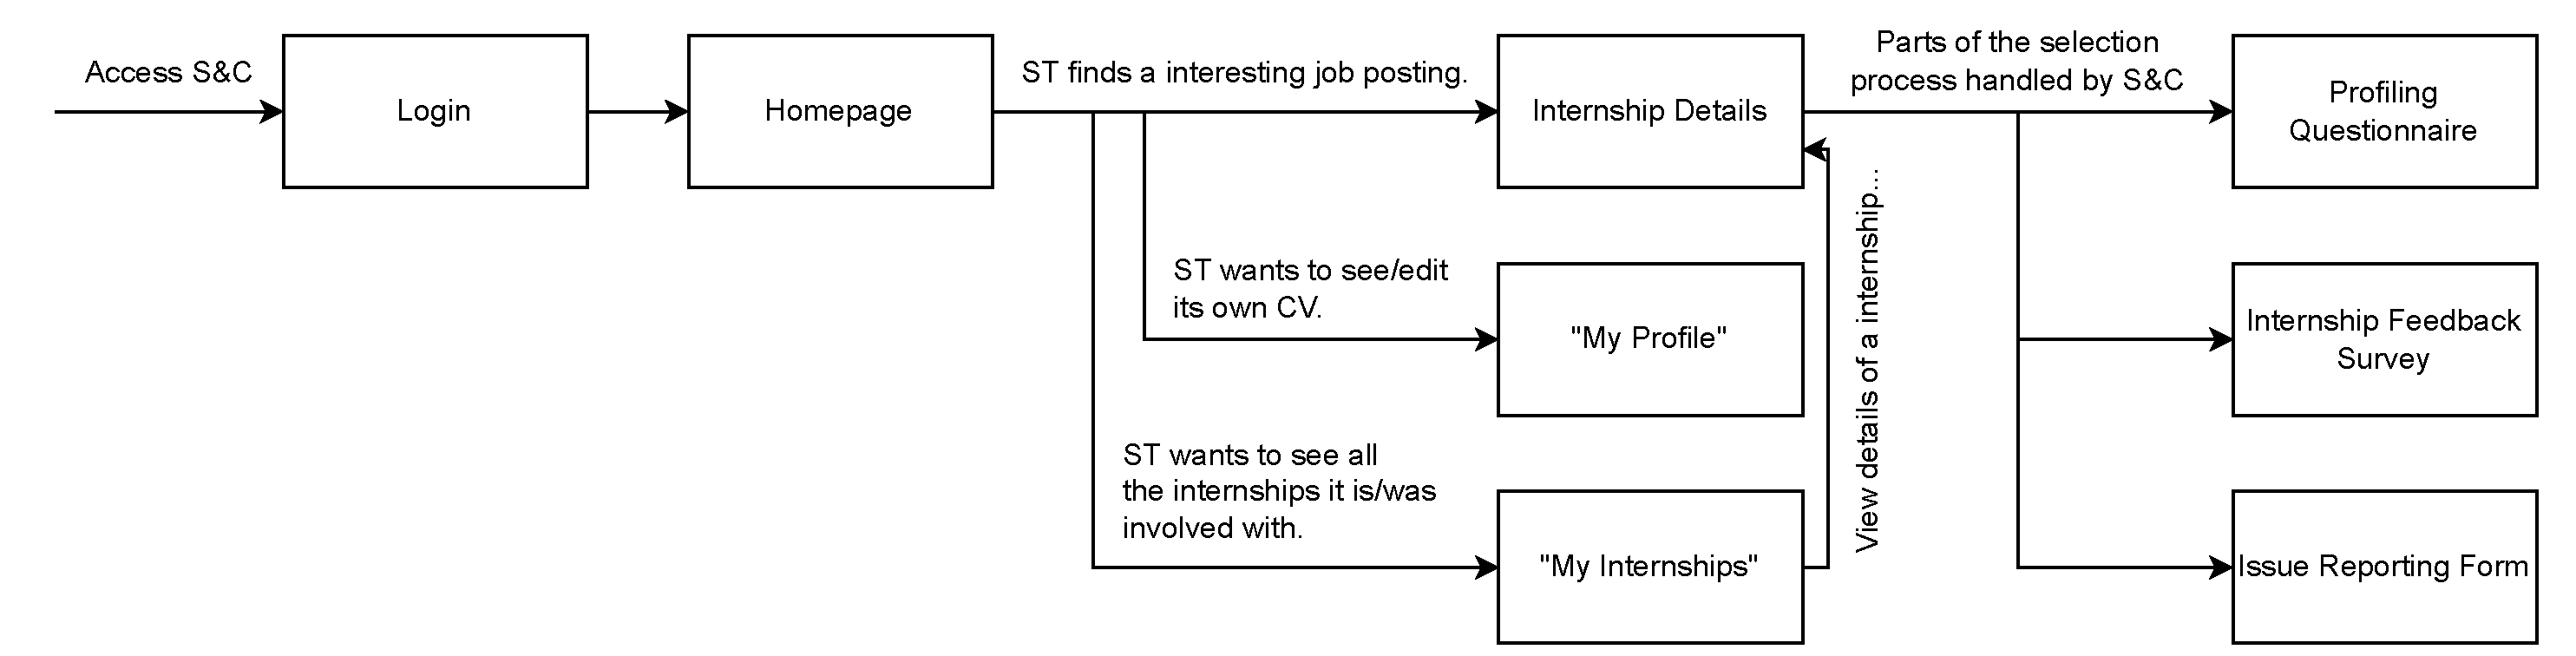
\includegraphics[width=0.9\textwidth]{Images/GUI/ST/Diagram.pdf}
    \caption{ST User Flow Diagram}
    \label{fig:st-user-flow-diagram}
\end{figure}

\par Here is presented the user flow diagram for the ST. The ST uses the "Login" page to authenticate and access S\&C
and then is redirected to the "Homepage". Here the user can discover new internships and view their details
("Internship Details"). The internship details page will allow the user to apply for the internship, access the
"Profiling Questionnaire", reports violations using the "Issue Reporting Form" and, once the internship is over,
access the "Internship Feedback Survey". By using the functions in the header the user can access their own profile
("My Profile"), view all the internships they have interacted with ("My Internships") and log out of the system.

\subsection{Login - ST}
\label{subsec:login-st}%

\begin{figure}[H]
    \centering
    \fbox{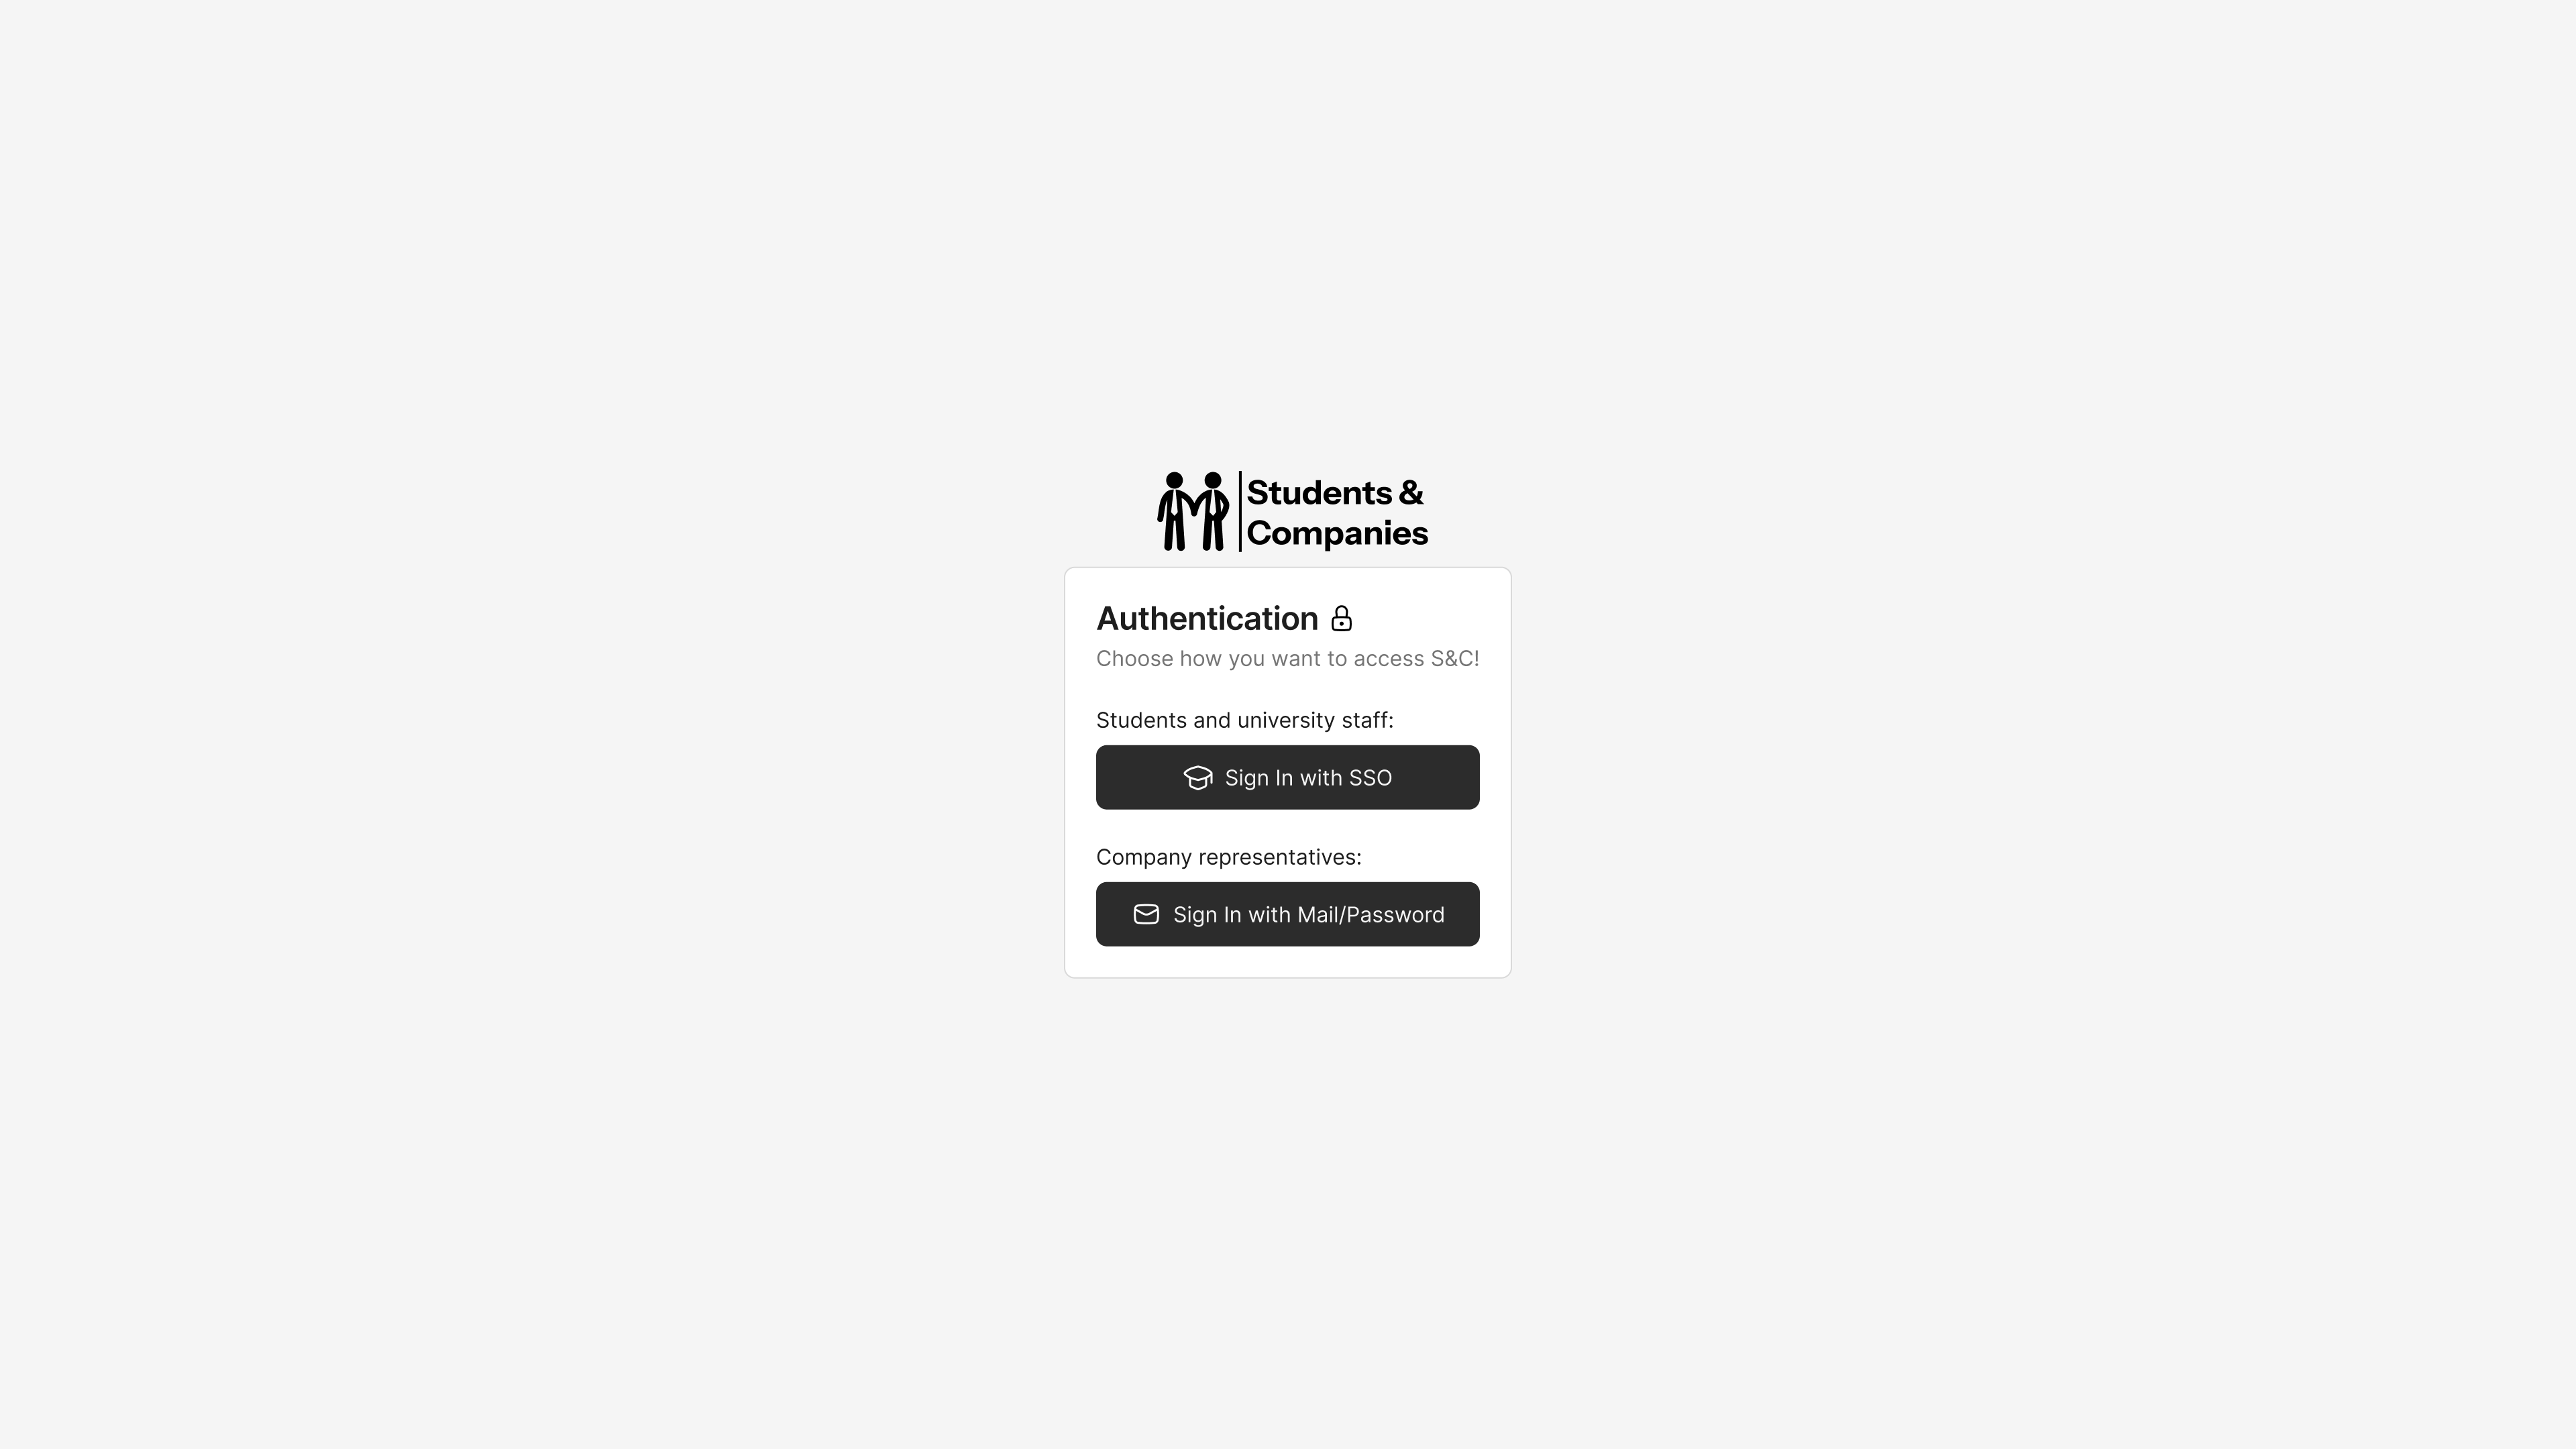
\includegraphics[width=1.0\textwidth]{Images/GUI/ST/Login - ST.png}}
    \caption{Login Page - ST}
    \label{fig:login-page-st}
\end{figure}

\par The login page is the first page the ST will see when accessing the S\&C platform. While ST and UN will use their
university authentication service to log in, a button to use standard credentials is also provided for CO users.

\subsection{Homepage - ST}
\label{subsec:homepage-st}%

\begin{figure}[H]
    \centering
    \fbox{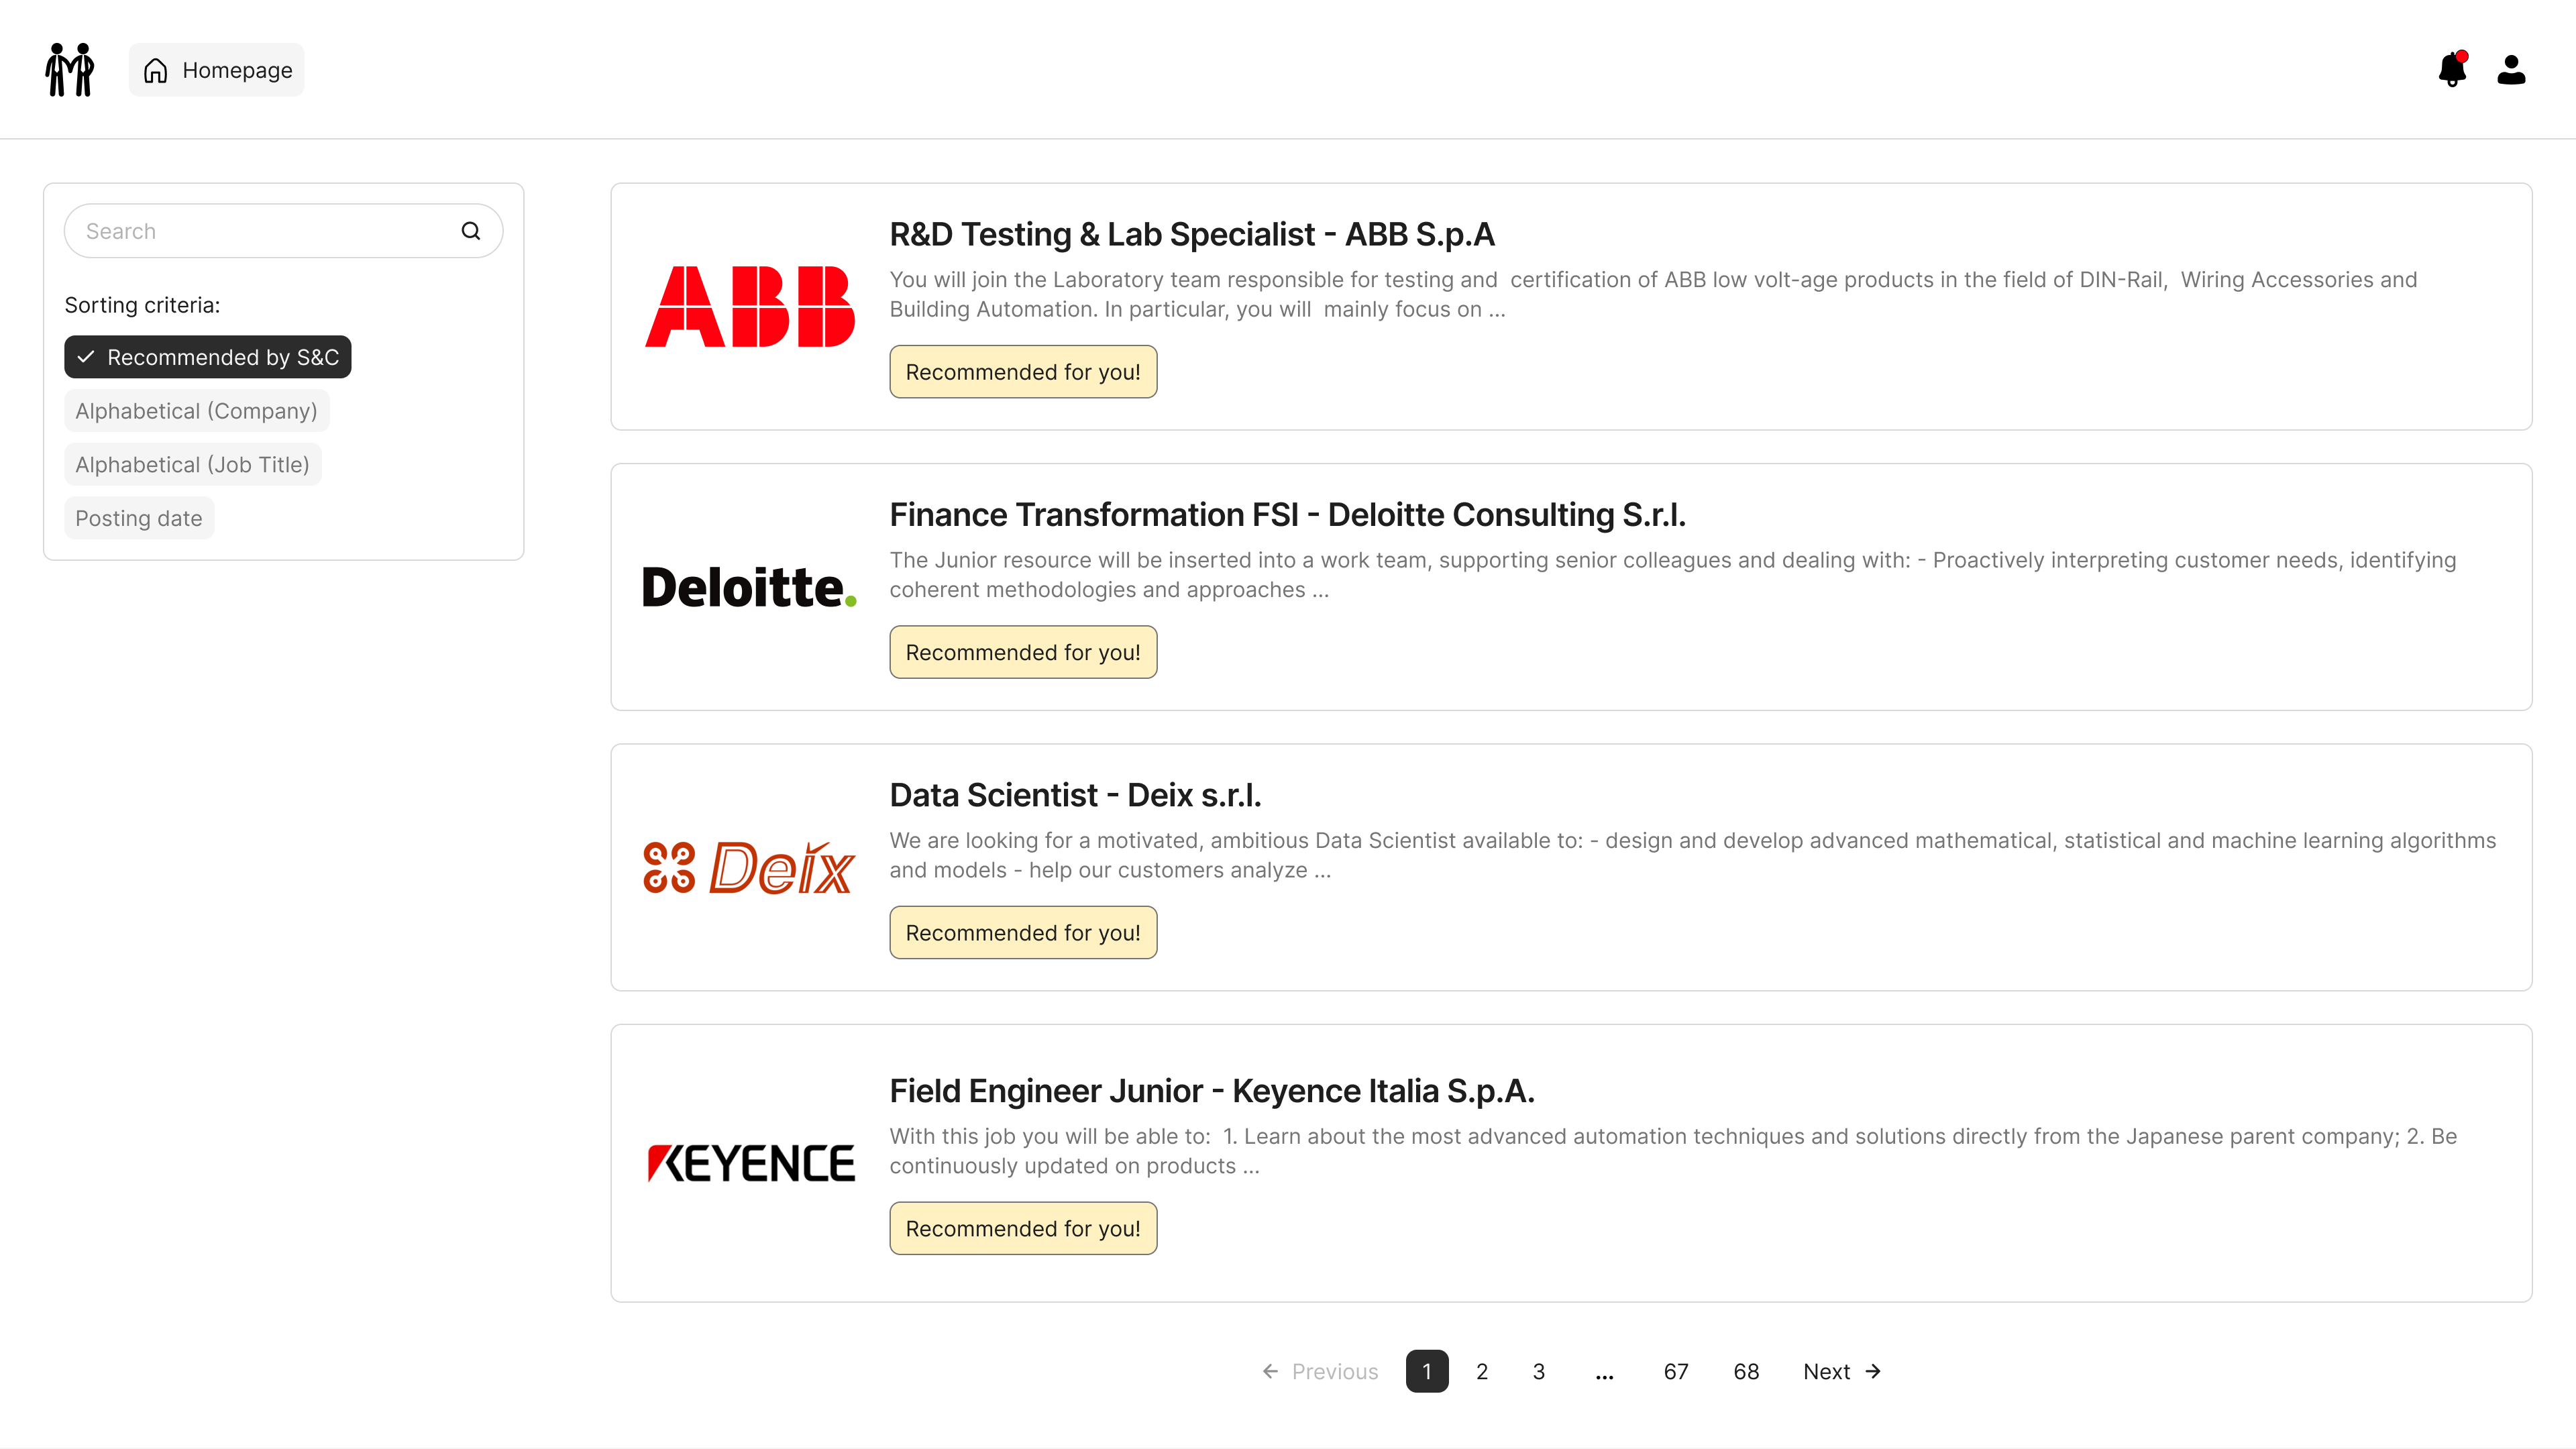
\includegraphics[width=1.0\textwidth]{Images/GUI/ST/Homepage - ST.png}}
    \caption{Homepage - ST}
    \label{fig:homepage-st}
\end{figure}

\par The homepage is the main page for the ST. Here the user can discover new internships and view their details. As
all the other pages, the header is present and allows the user to access their profile, view their internships and
log out. Also, a notification submenu is present to show the user any new notifications in case they missed the email.

\par Appropriate filters are provided to allow the user to search for internships based on their preferences.

\begin{figure}[H]
    \centering
    \fbox{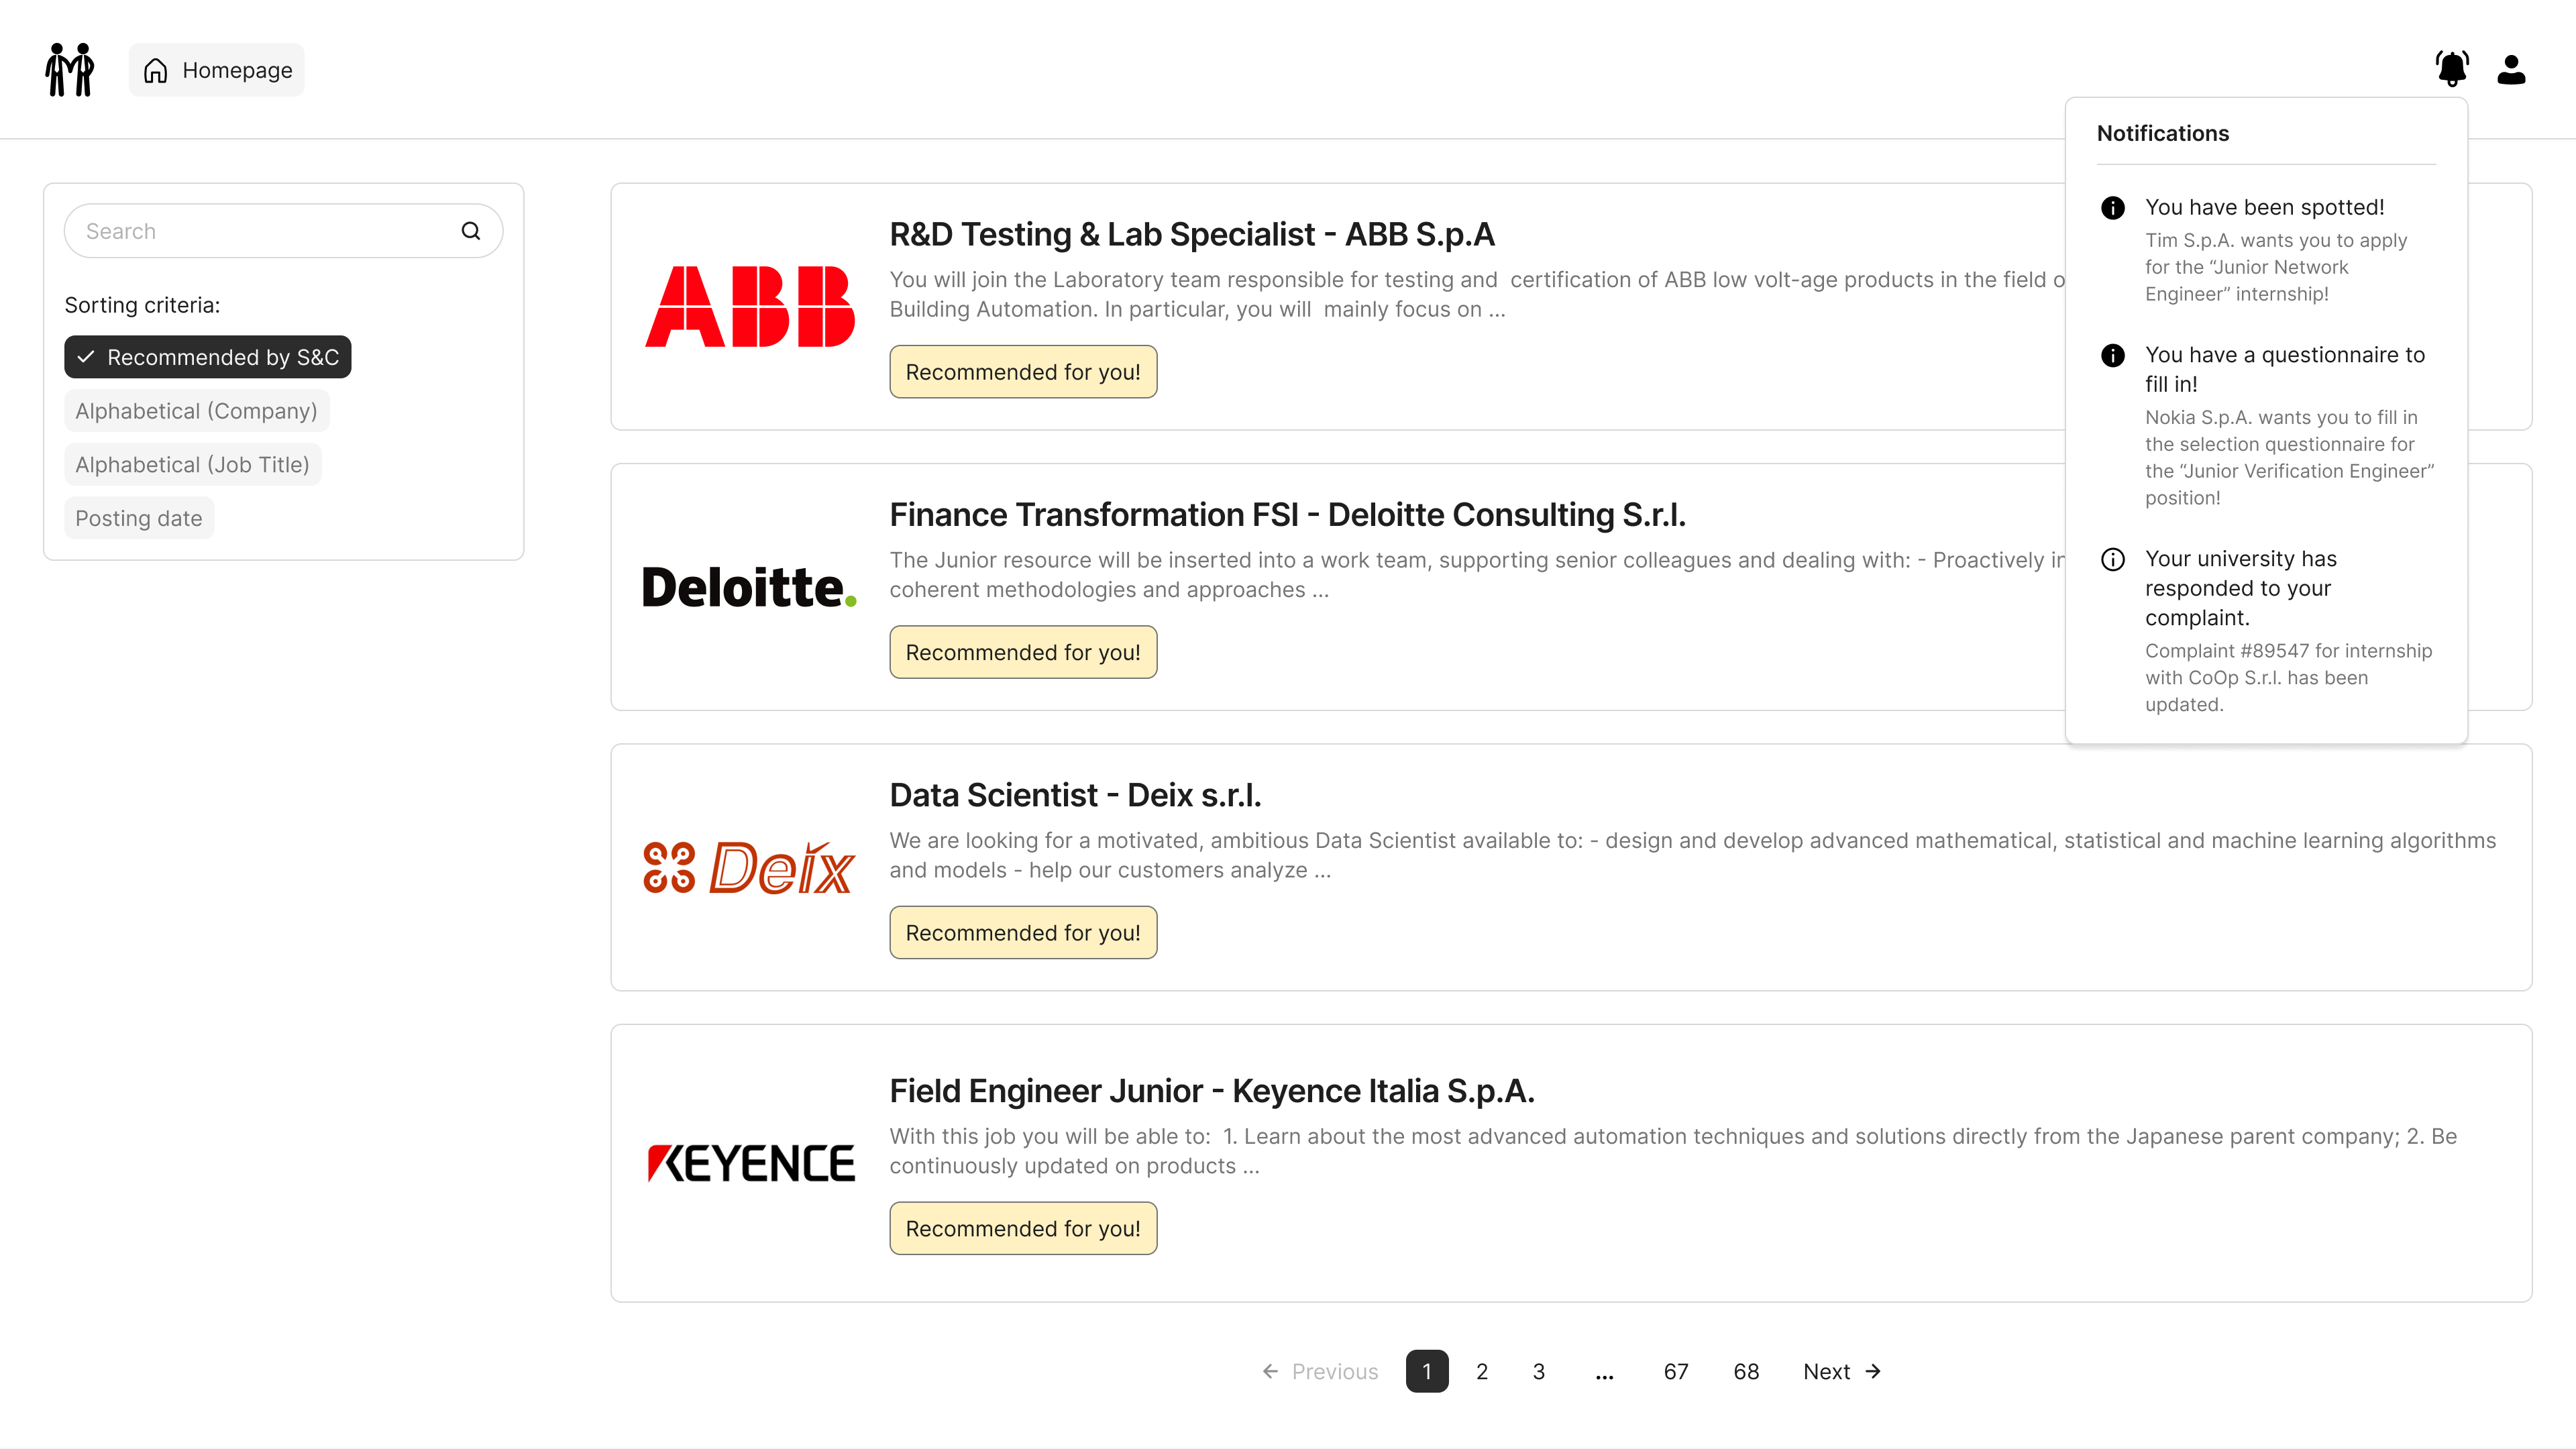
\includegraphics[width=1.0\textwidth]{Images/GUI/ST/Homepage - ST - Notification.png}}
    \caption{Homepage - ST - Notification}
    \label{fig:homepage-st-notification}
\end{figure}

\begin{figure}[H]
    \centering
    \fbox{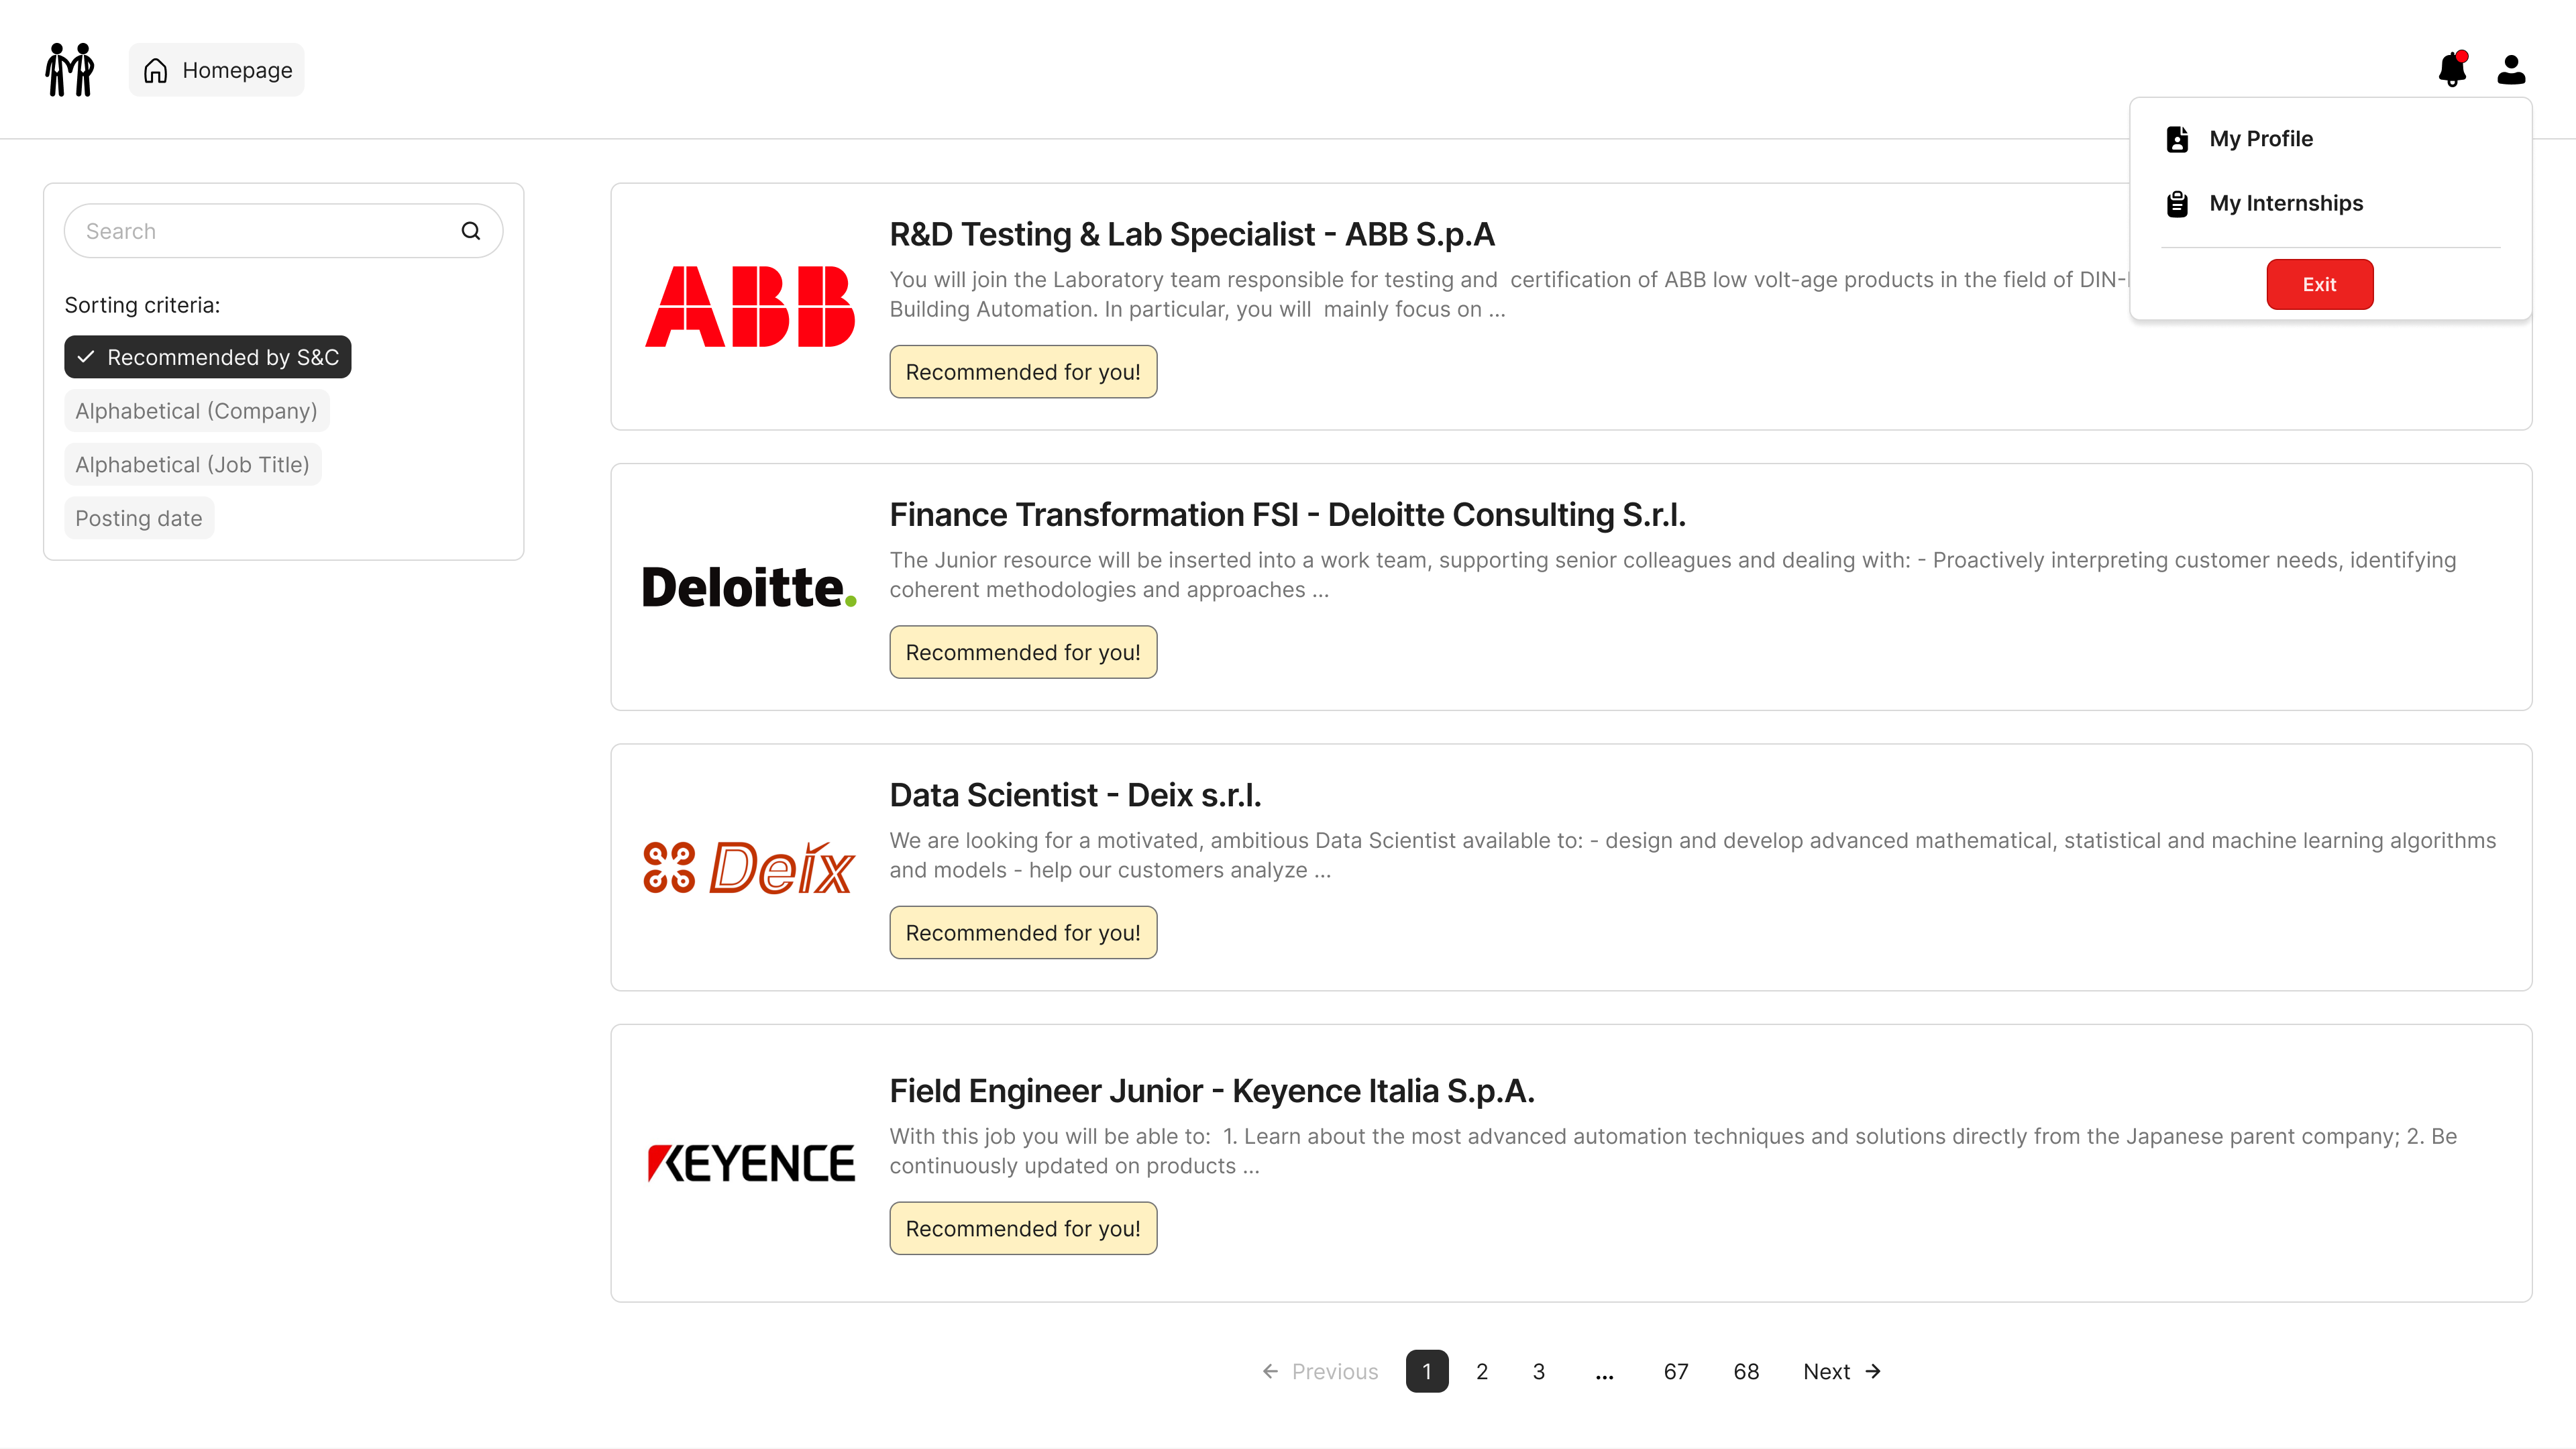
\includegraphics[width=1.0\textwidth]{Images/GUI/ST/Homepage - ST - Profile.png}}
    \caption{Homepage - ST - Profile}
    \label{fig:homepage-st-profile}
\end{figure}

\subsection{"My Internships" - ST}
\label{subsec:my-internships-st}%

\begin{figure}[H]
    \centering
    \fbox{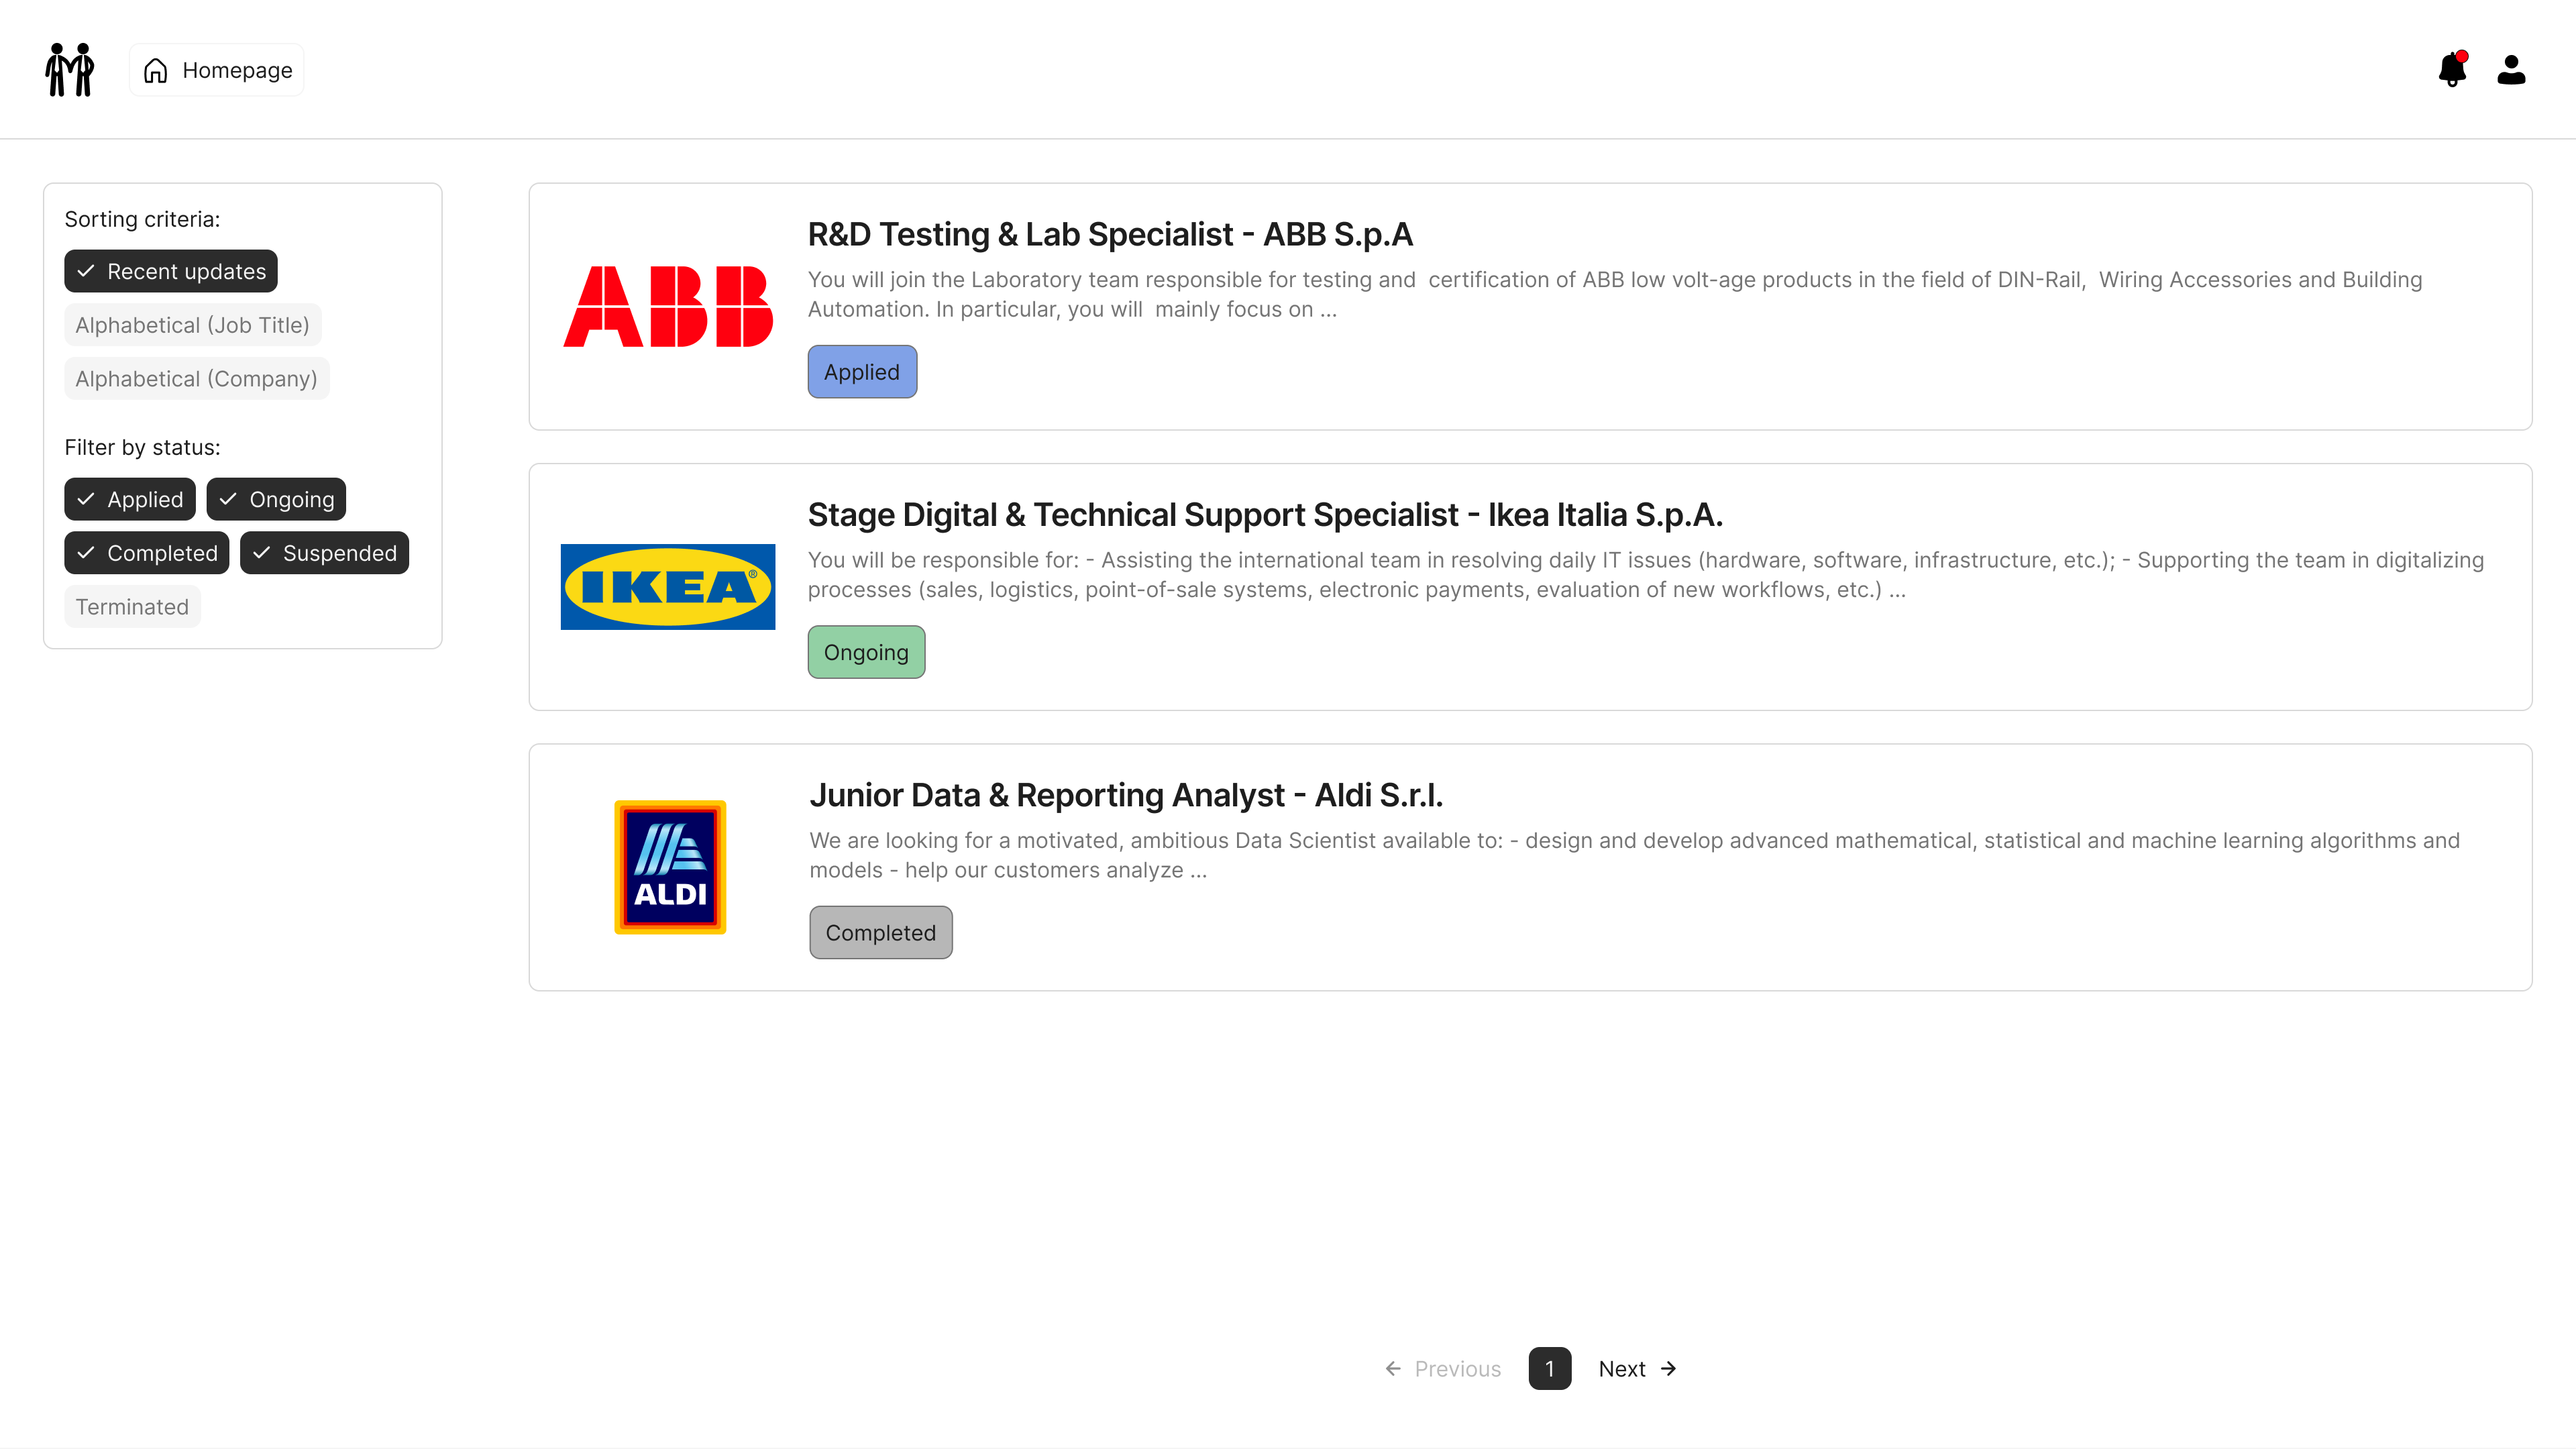
\includegraphics[width=1.0\textwidth]{Images/GUI/ST/My Internships - ST.png}}
    \caption{"My Internships" - ST}
    \label{fig:my-internships-st}
\end{figure}

\par The "My Internships" page allows the ST to view all the internships they have interacted with. It is similar to
the homepage and as such filters are provided.

\subsection{"Profile" - ST}
\label{subsec:profile-st}%

\begin{figure}[H]
    \centering
    \fbox{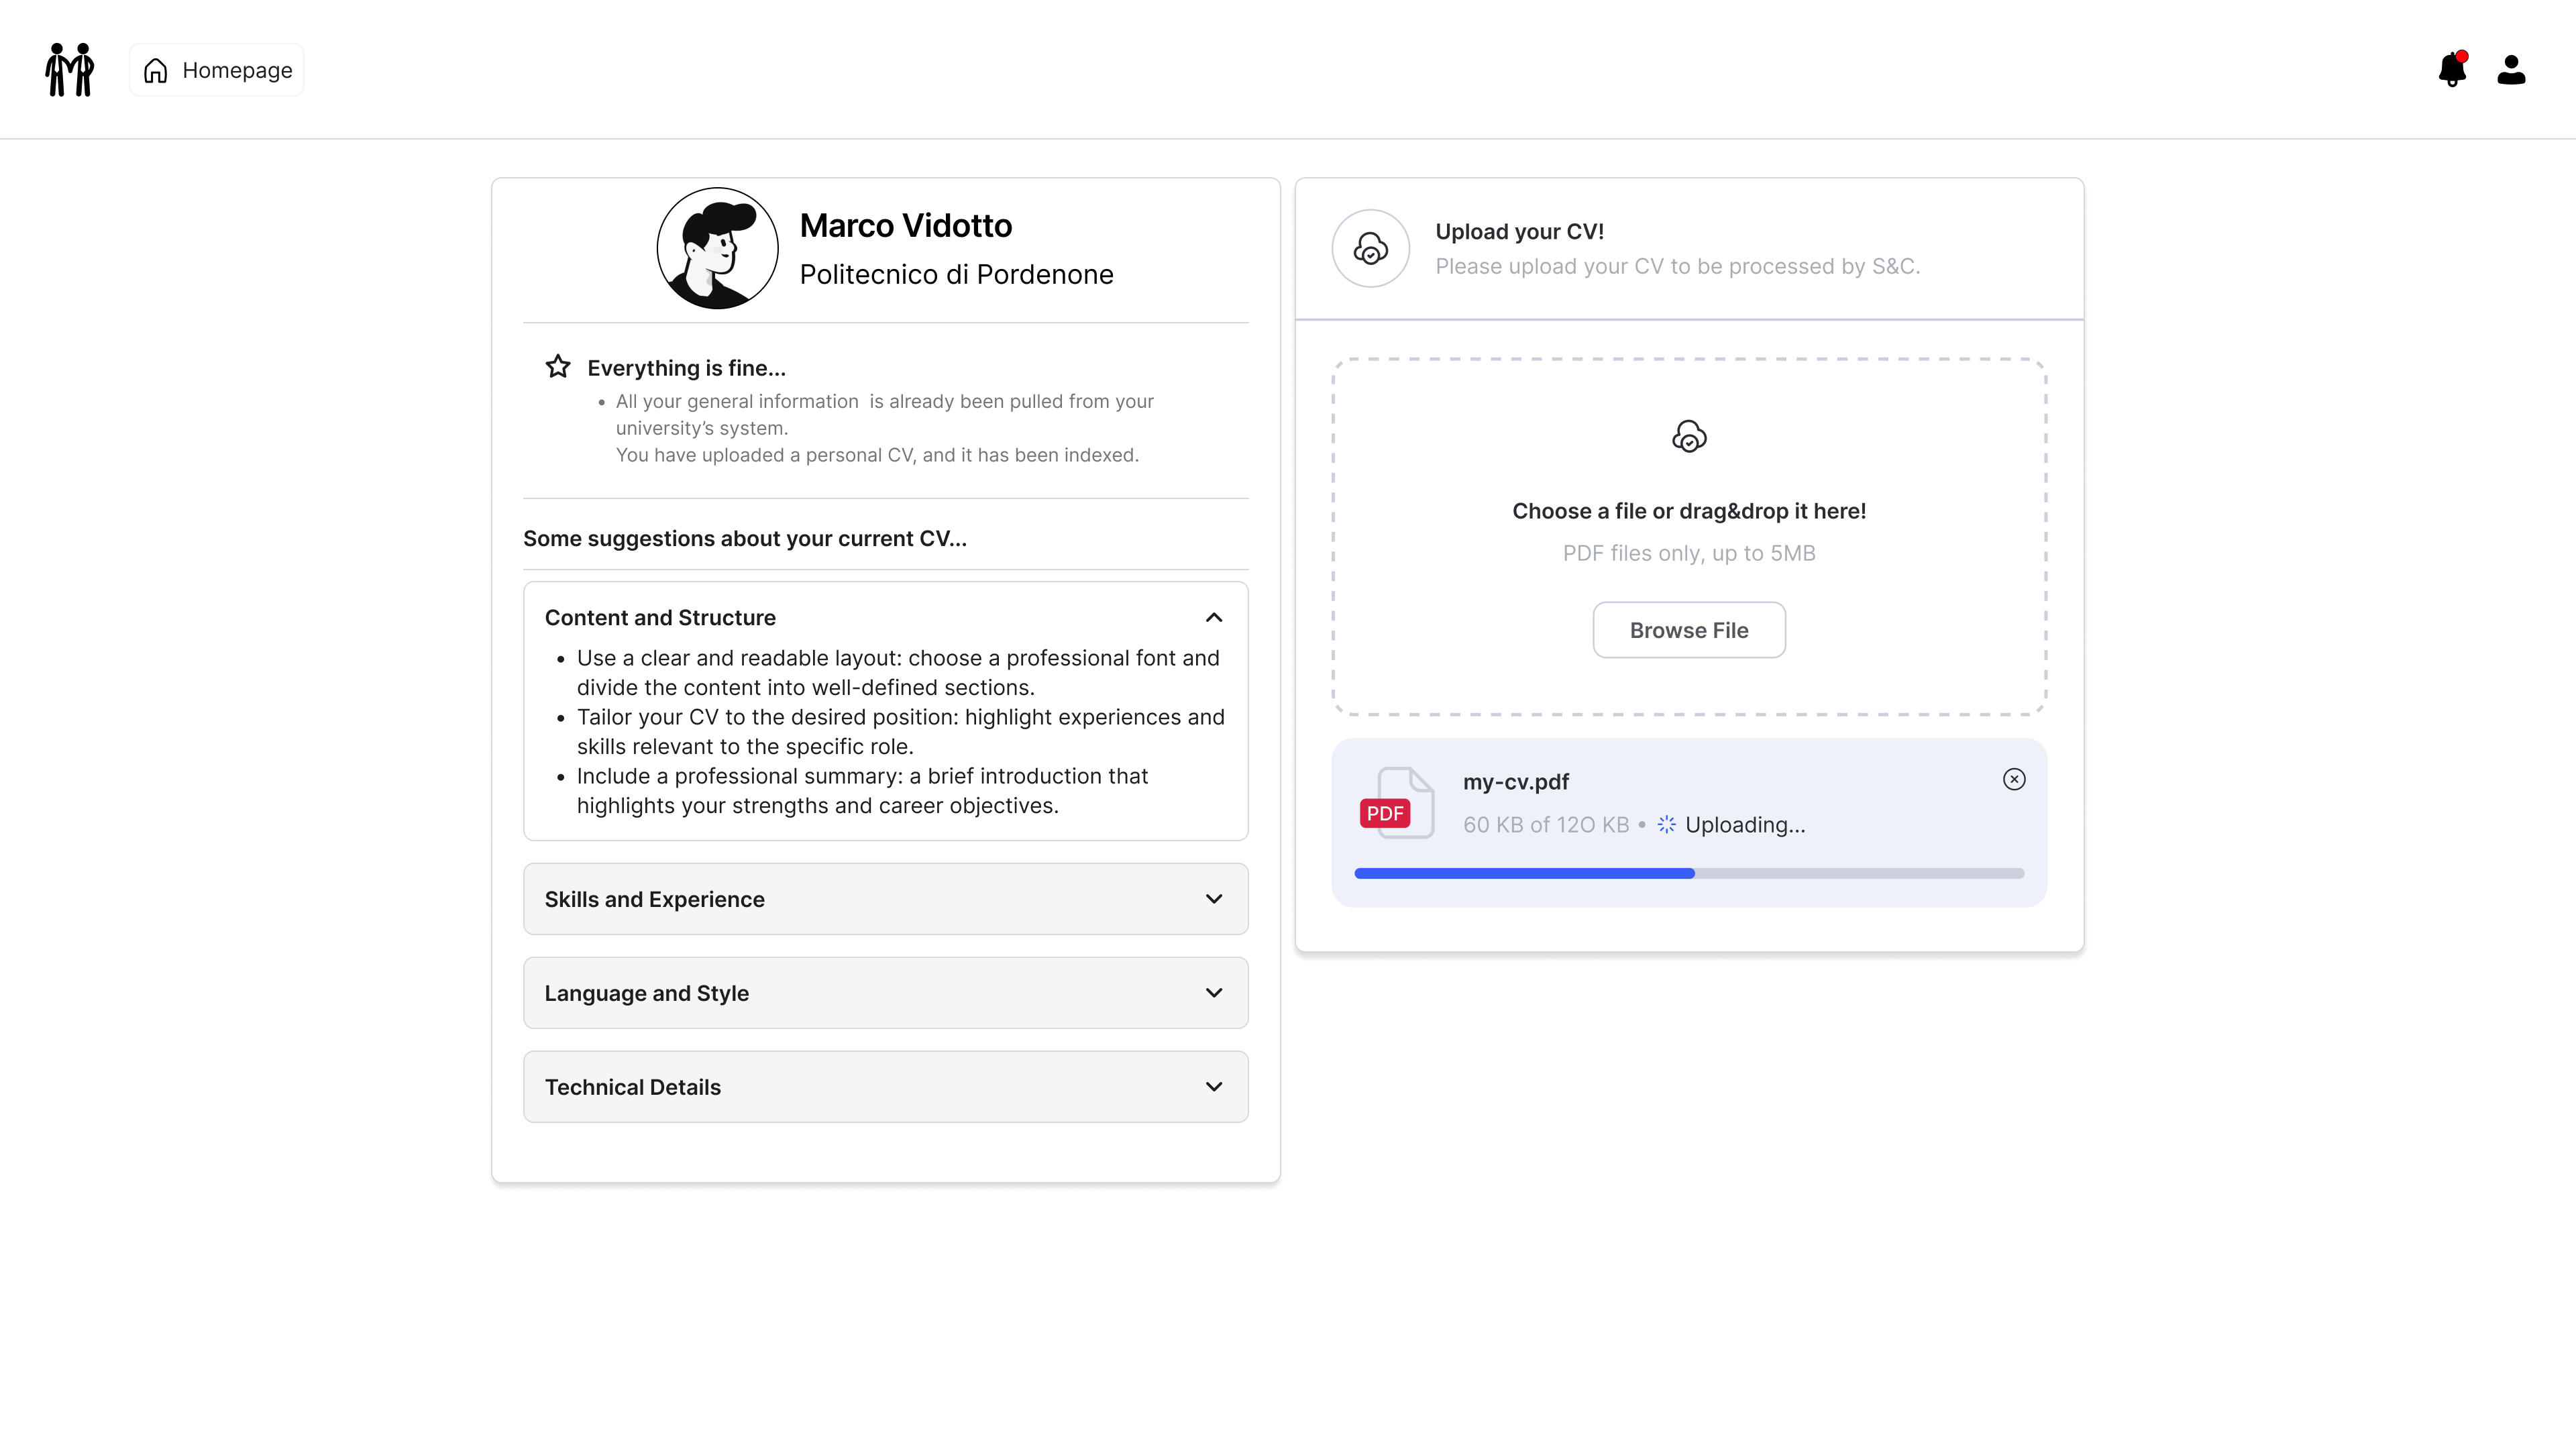
\includegraphics[width=1.0\textwidth]{Images/GUI/ST/Profile - ST.png}}
    \caption{"Profile" - ST}
    \label{fig:profile-st}
\end{figure}

\par The "Profile" page allows the ST to update their personal information by uploading a new CV (PDF only!).
Suggestions on how to improve the CV are also provided.

\subsection{"Internship Details" - ST}

\begin{figure}[H]
    \centering
    \fbox{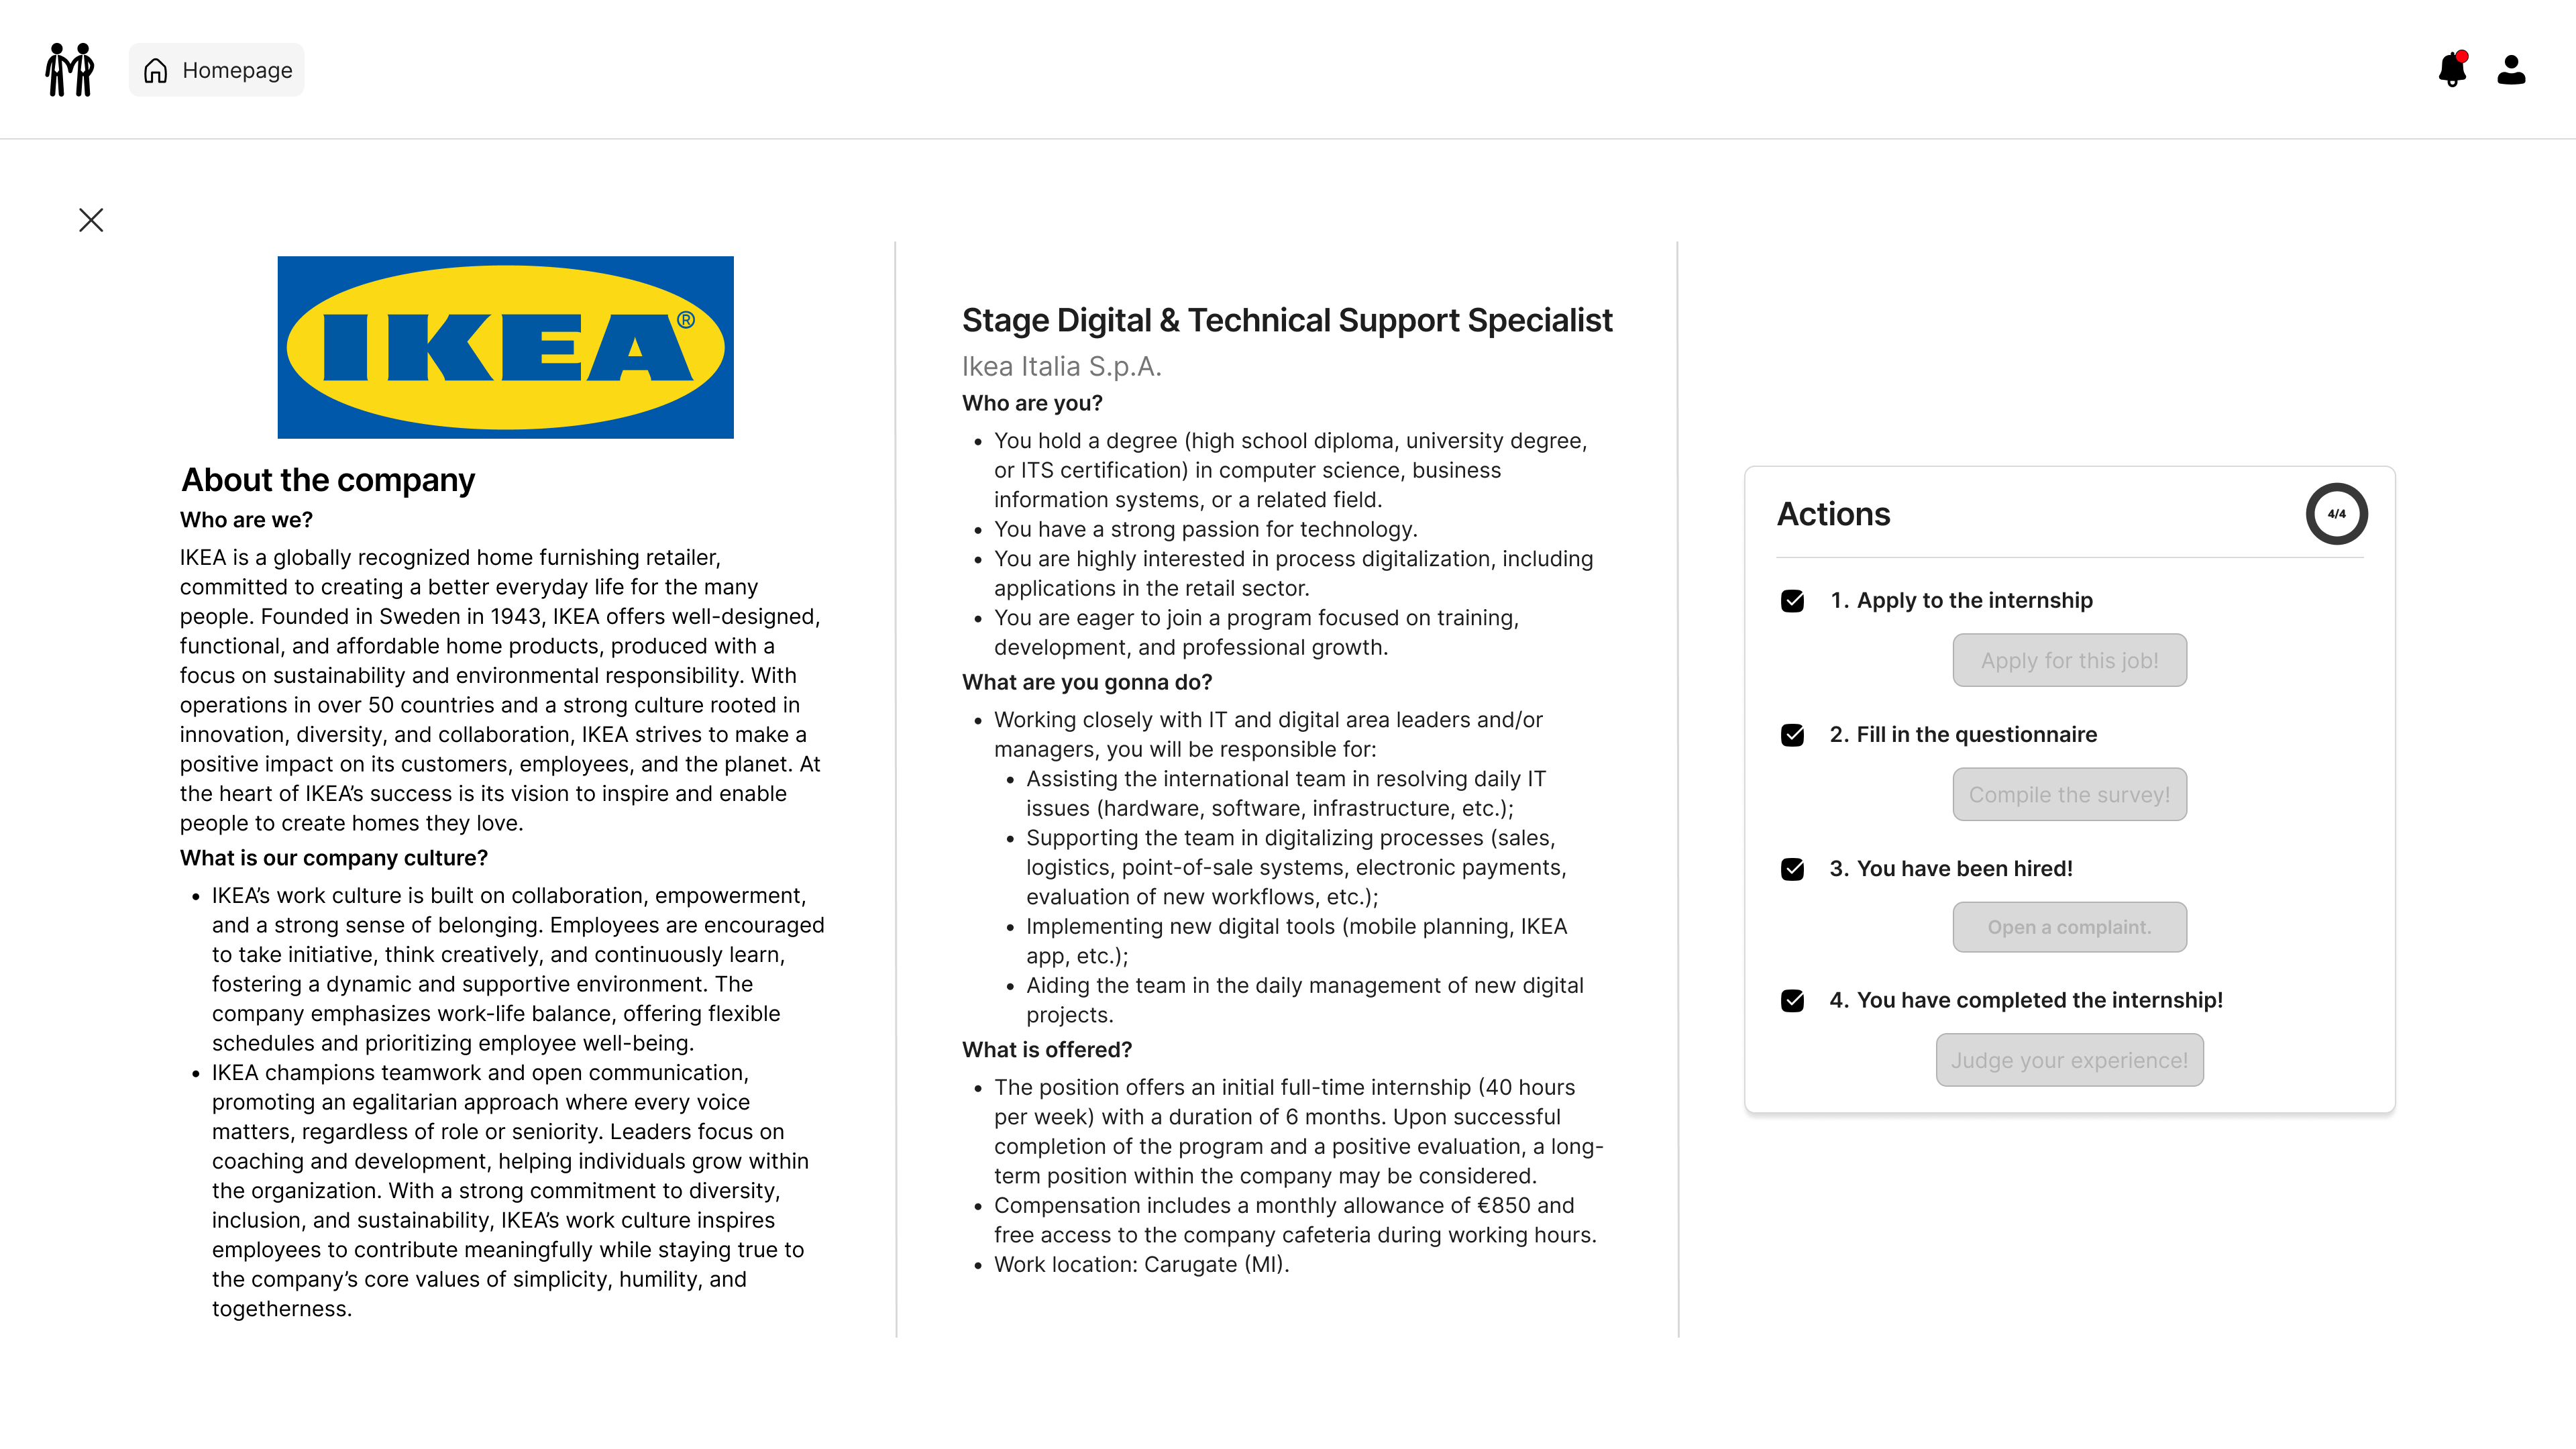
\includegraphics[width=1.0\textwidth]{Images/GUI/ST/Internship Details - Completed - ST.png}}
    \caption{"Internship Details" - ST}
    \label{fig:internship-details-st}
\end{figure}

\par The "Internship Details" page allows the ST to view all the details of an internship and the company that is
offering it. The ST can apply for the internship, access the "Profiling Questionnaire", report violations using the
"Issue Reporting Form" and, once the internship is over, access the "Internship Feedback Survey".

\par The various functions are enabled or disabled based on the status of the internship. A progress bar is also
present to show the progression of the hiring process.

\par For simplicity, here is presented the page for a completed
internship; from this example will it be easy to infer how the page will look like for all the various stages of the
hiring process.

\subsection{"Profiling Questionnaire" - ST}
\label{subsec:profiling-questionnaire-st}%

\begin{figure}[H]
    \centering
    \fbox{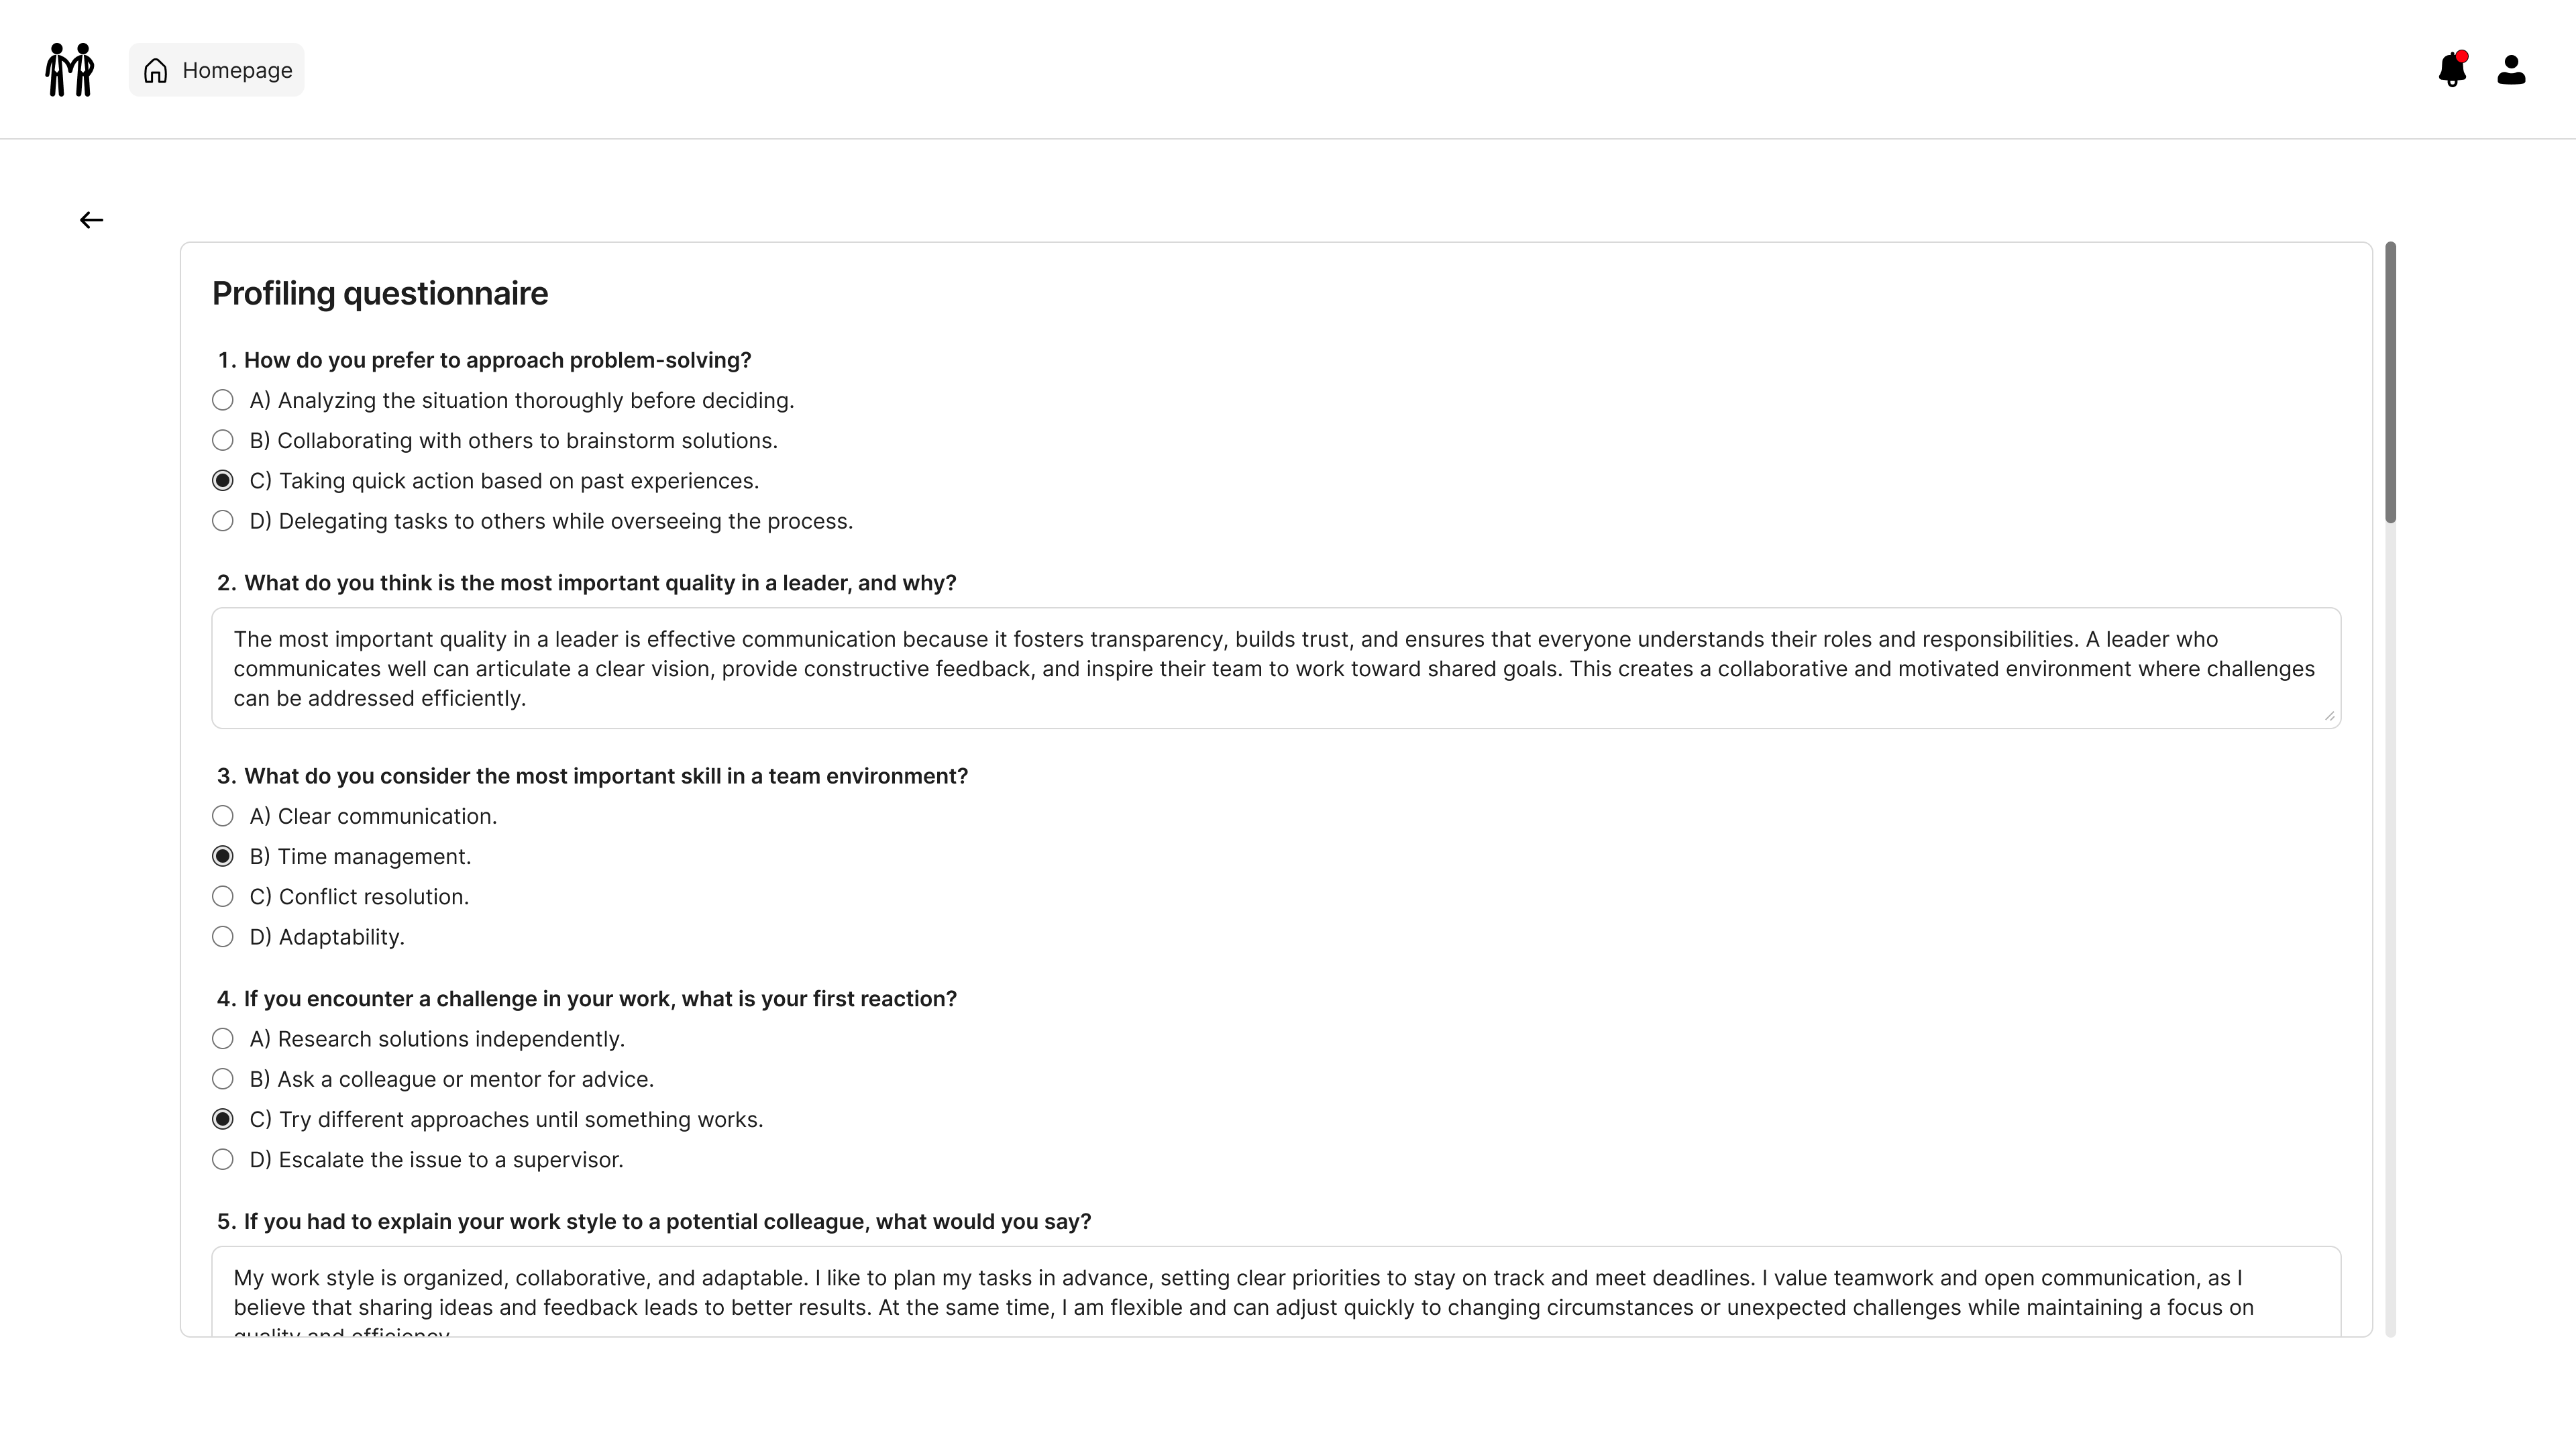
\includegraphics[width=1.0\textwidth]{Images/GUI/ST/Profiling Questionnaire - ST.png}}
    \caption{"Profiling Questionnaire" - ST}
    \label{fig:profiling-questionnaire-st}
\end{figure}

\par The "Profiling Questionnaire" page allows the ST to fill in a questionnaire to provide the company with more
information about themselves. The various questions will be automatically graded by the system to provide the
company with a synthetic evaluation of the ST. The questions will be provided manually by the CO.

\subsection{"Issue Reporting Form" - ST}
\label{subsec:issue-reporting-form-st}%

\begin{figure}[H]
    \centering
    \fbox{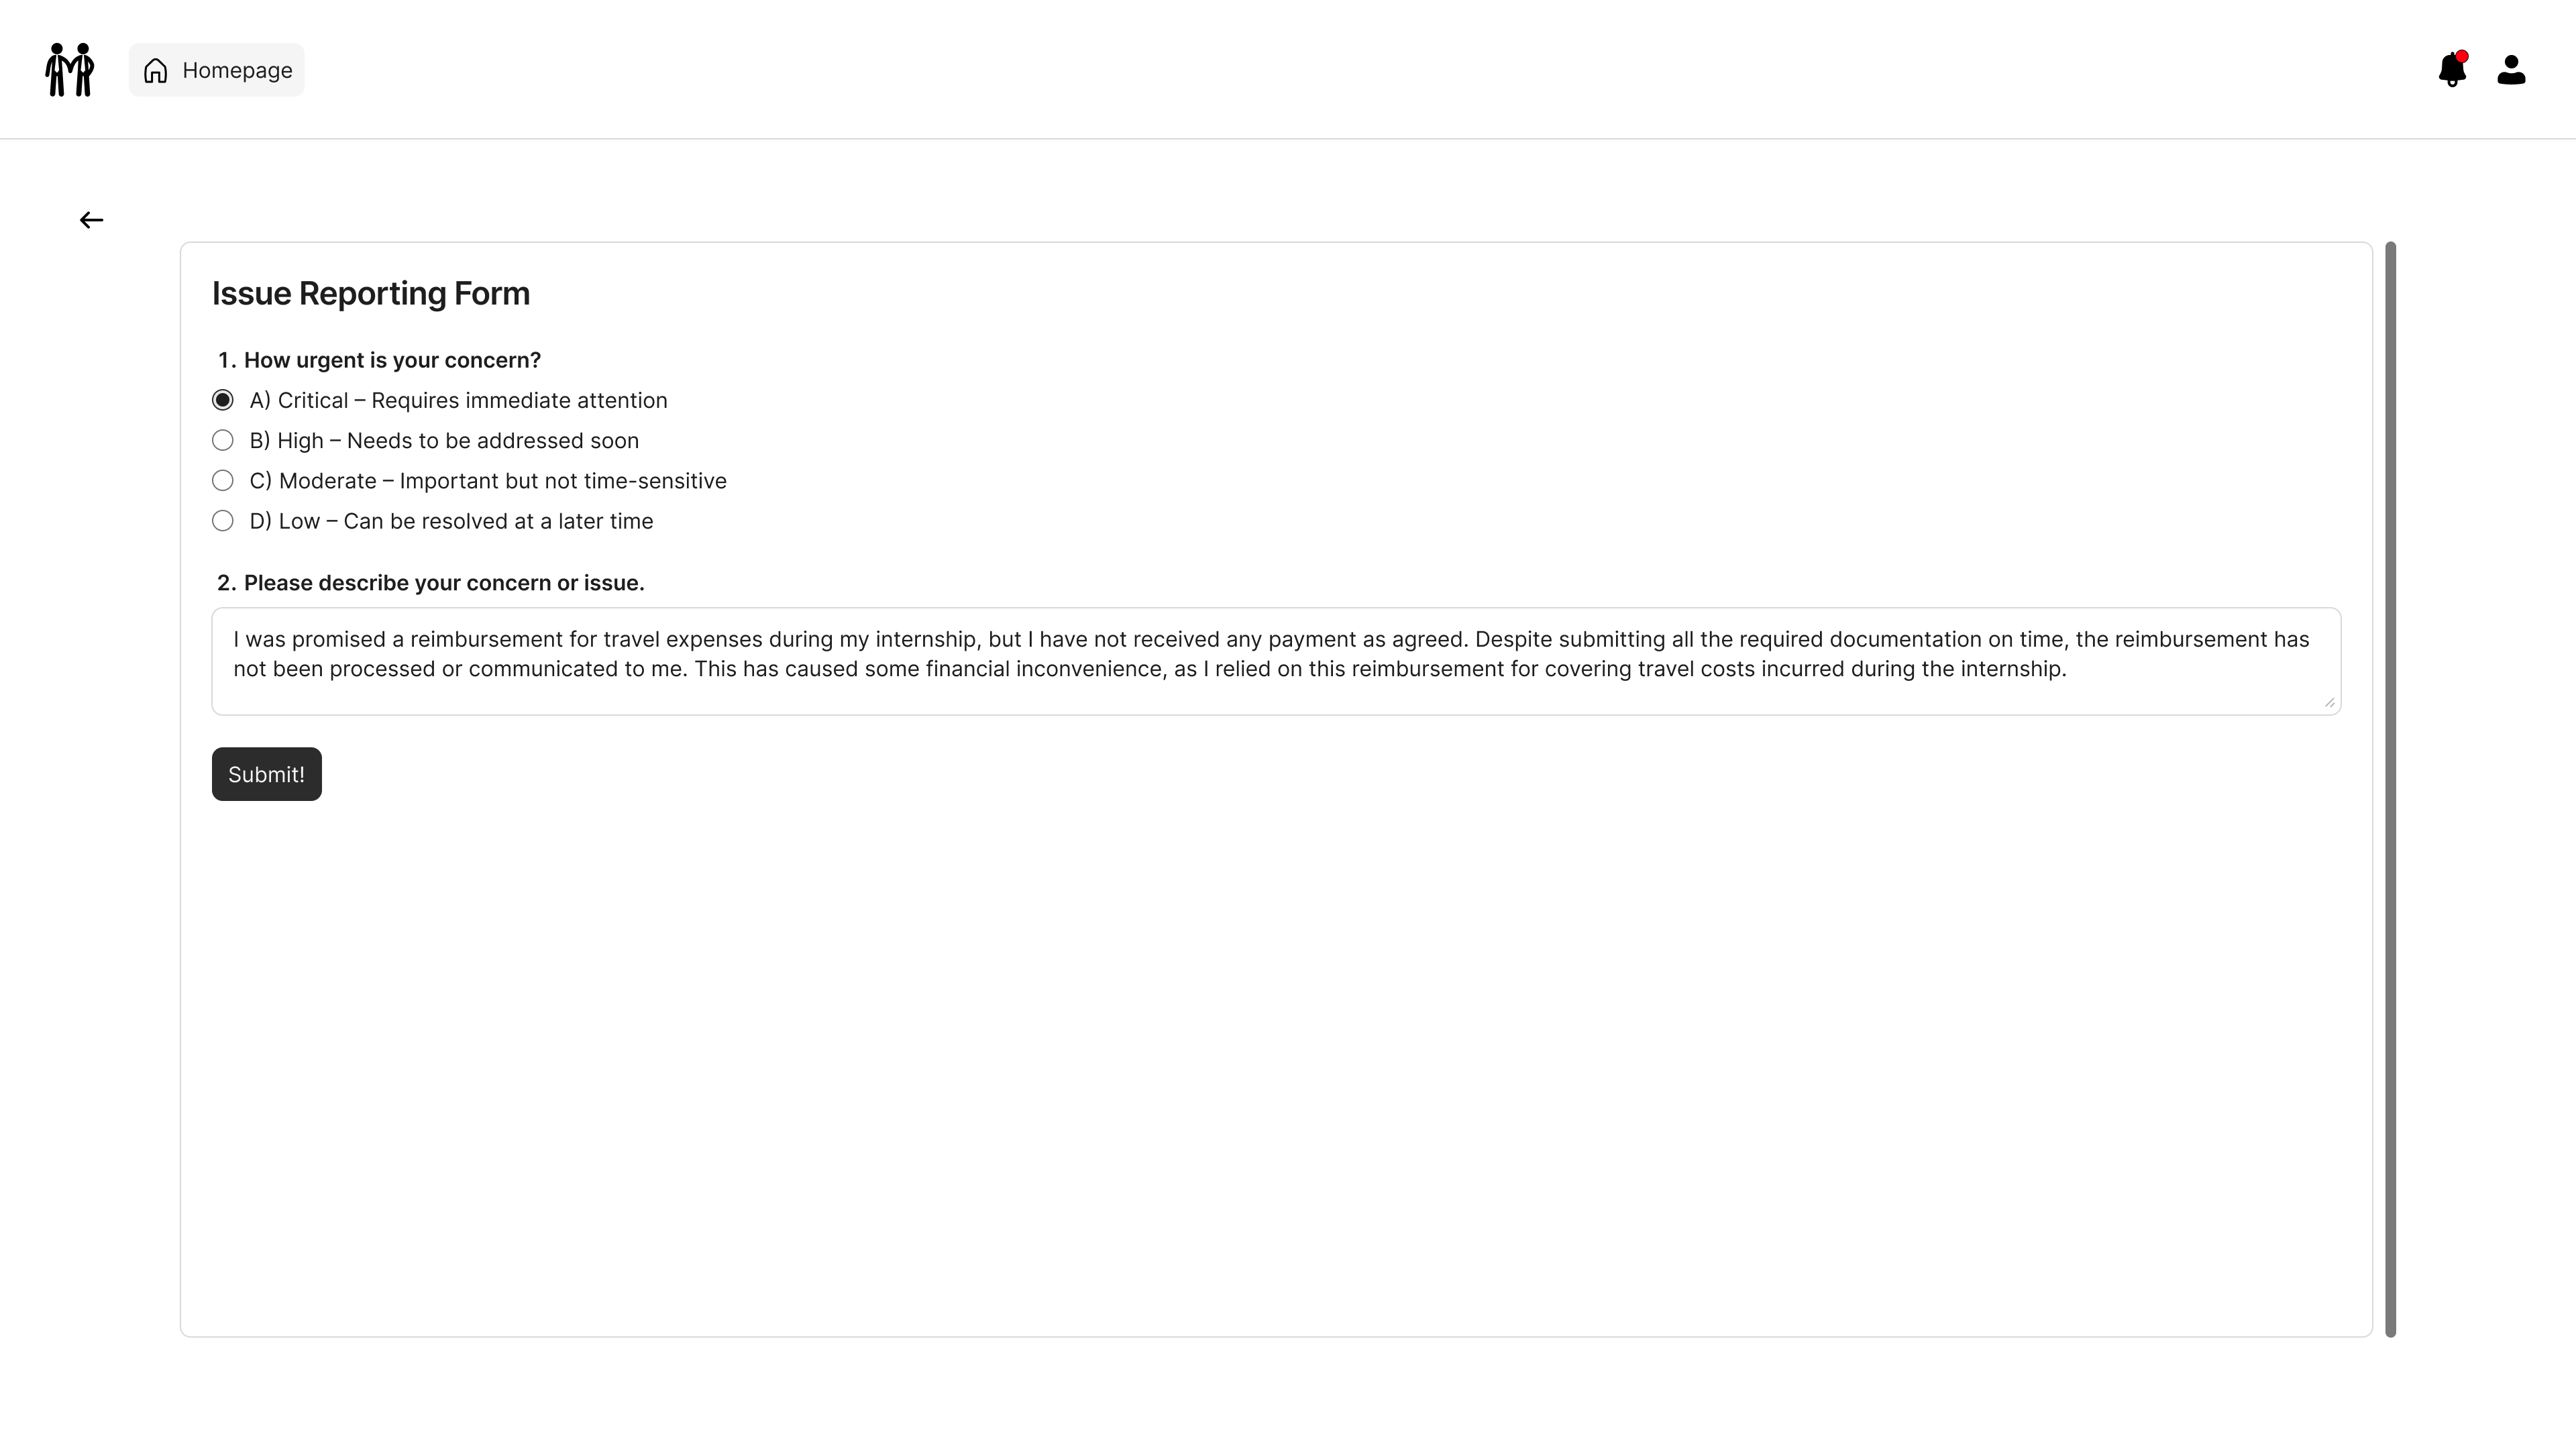
\includegraphics[width=1.0\textwidth]{Images/GUI/ST/Issue Reporting Form - ST.png}}
    \caption{"Issue Reporting Form" - ST}
    \label{fig:issue-reporting-form-st}
\end{figure}

\par The "Issue Reporting Form" page allows the ST to report any violations they have encountered during the
internship. The form is simple and allows the user to provide a description of the violation and any evidence they
have. The form is then sent to the company and the UN to evaluate the situation.

\par The user himself can choose the urgency of their issue.

\subsection{"Internship Feedback Survey" - ST}
\label{subsec:internship-feedback-survey-st}%

\begin{figure}[H]
    \centering
    \fbox{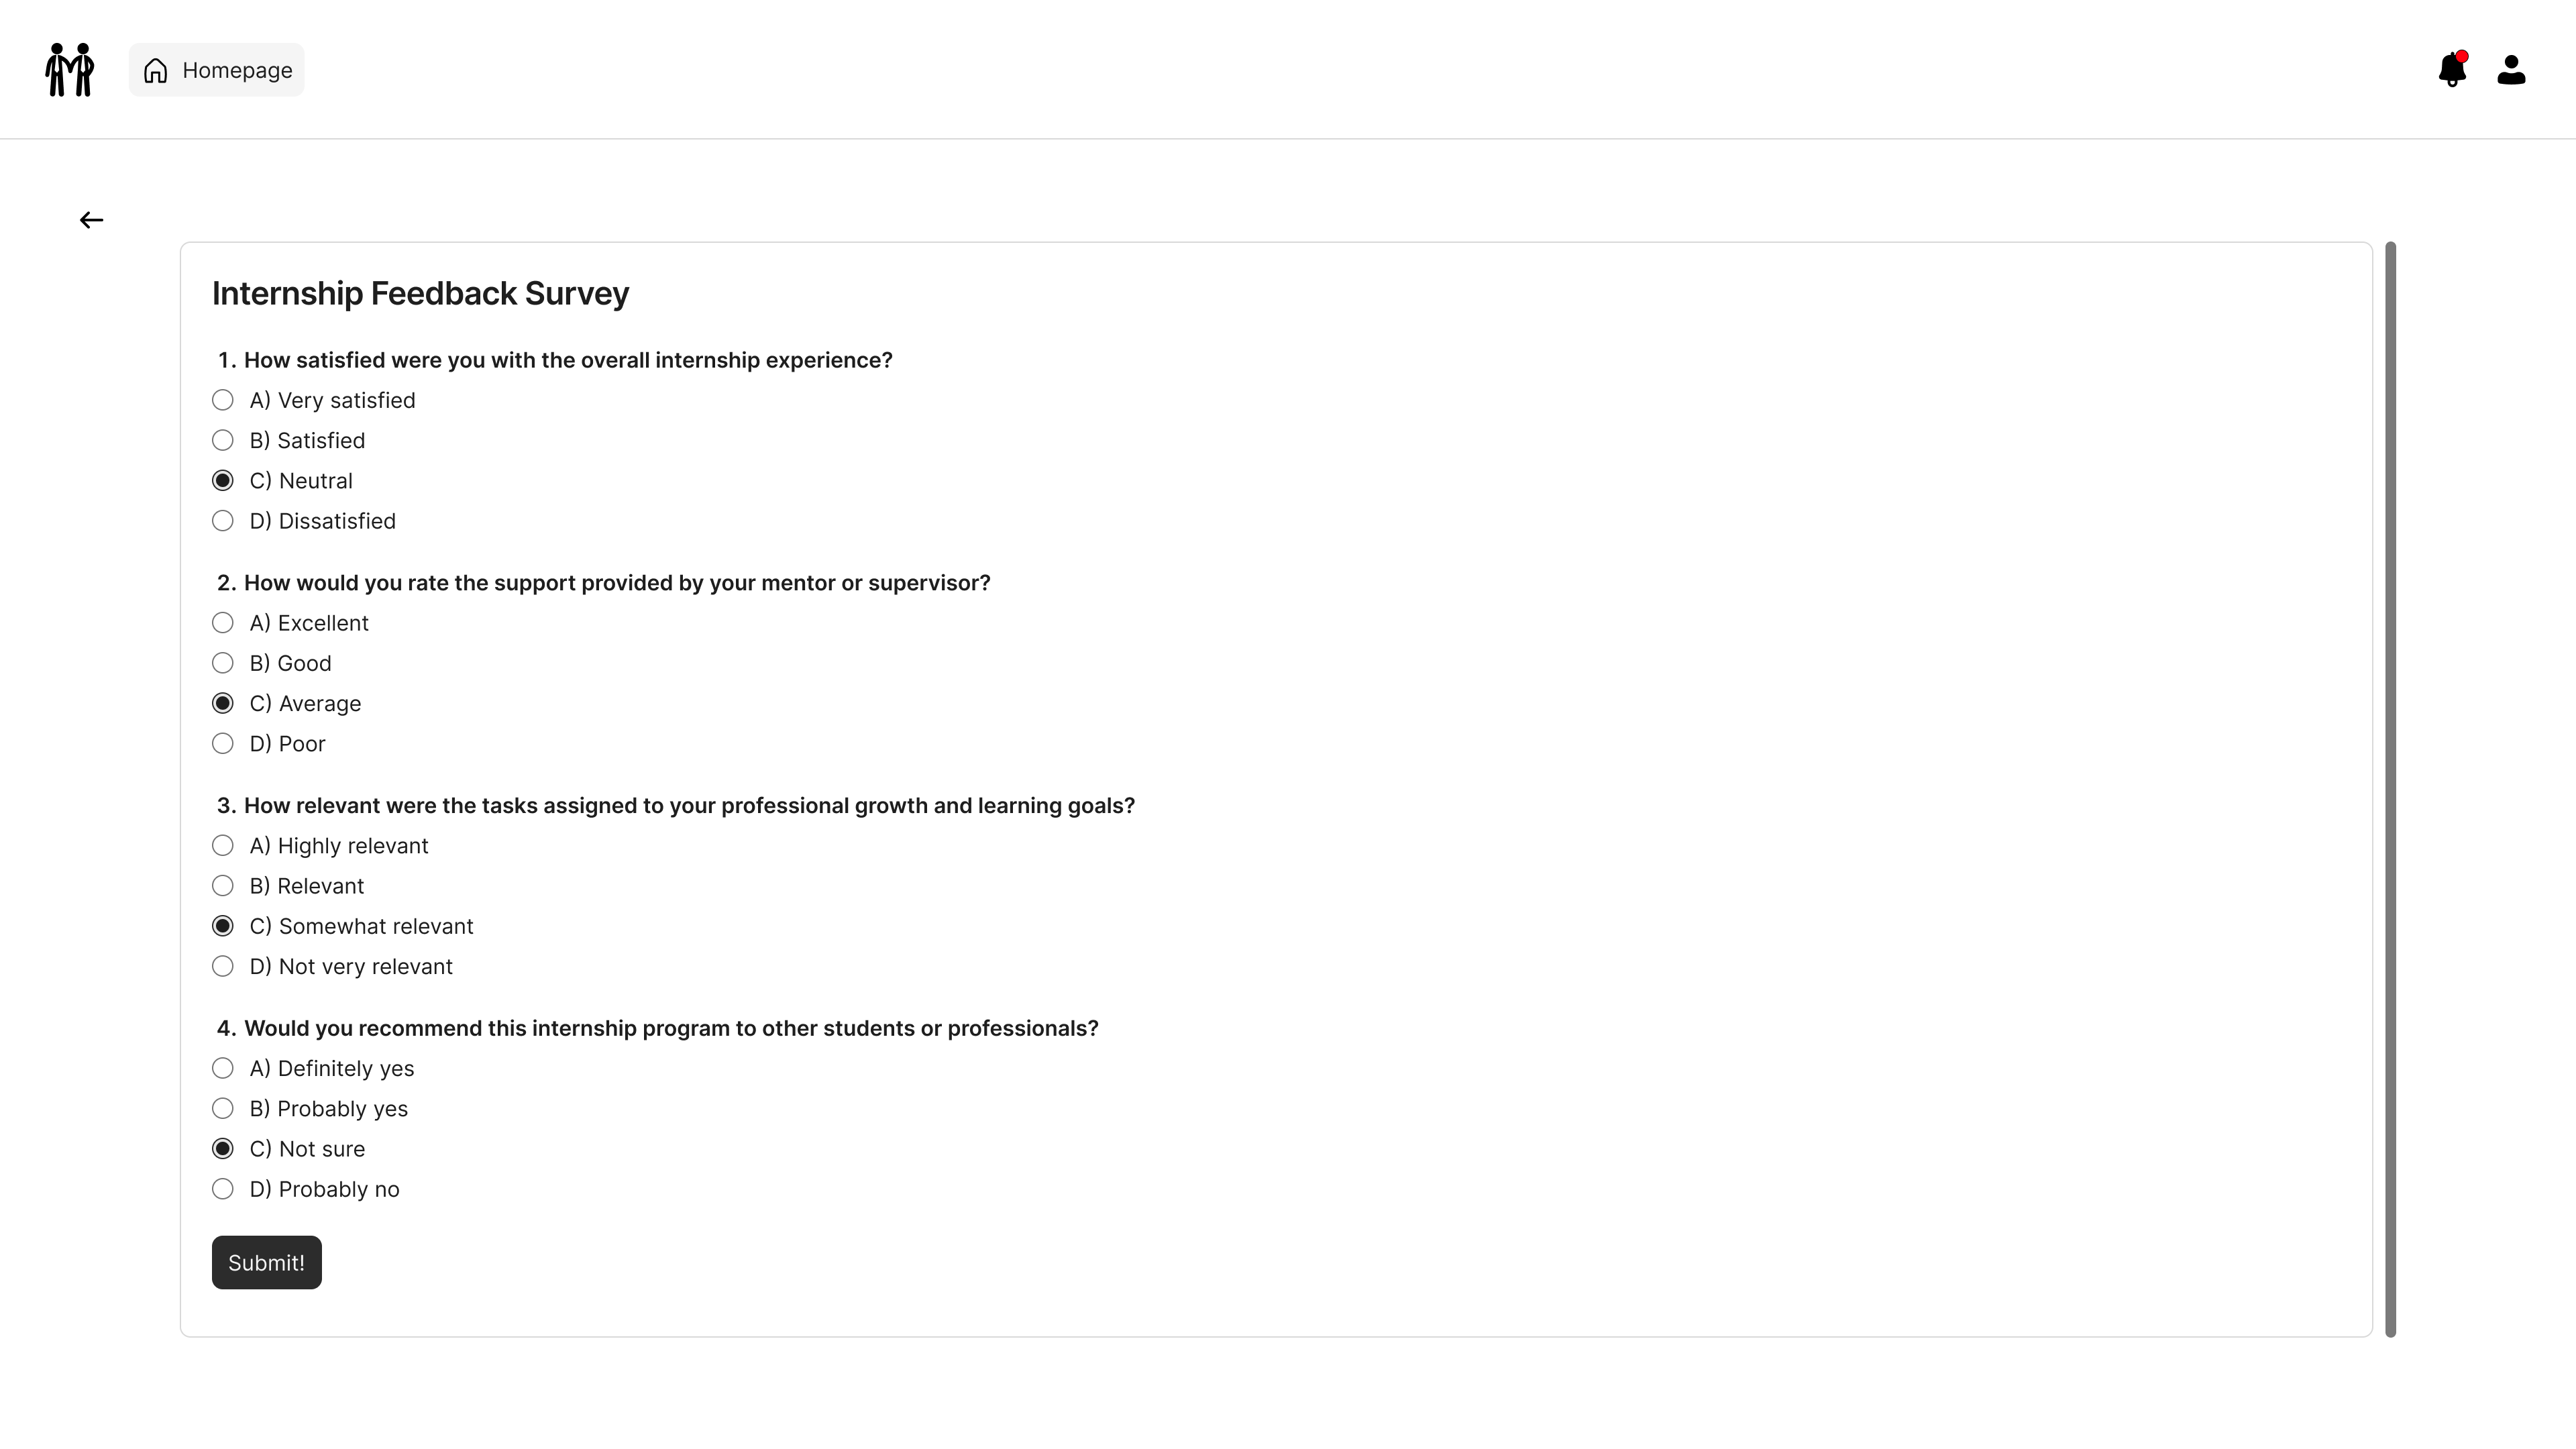
\includegraphics[width=1.0\textwidth]{Images/GUI/ST/Internship Feedback Survey - ST.png}}
    \caption{"Internship Feedback Survey" - ST}
    \label{fig:internship-feedback-survey-st}
\end{figure}

\par The "Internship Feedback Survey" page allows the ST to provide a final evaluation on the internship. S\&C and UN
will use this information to improve the quality of the internships and the platform.
